\documentclass[a4paper,twoside,12pt]{report}
\usepackage[pdftex]{graphicx}
\usepackage{tocloft}
%
\usepackage[smaller]{acronym}
\usepackage{amsfonts}
\usepackage{amsmath}
\usepackage{atlasphysics}
\usepackage{bbold}
\usepackage{booktabs}
\usepackage[pdftex,color]{changebar}
\usepackage{fancyhdr}
\usepackage{hyperref}
\usepackage{lineno}
\usepackage{mathrsfs}
\usepackage{multirow}
\usepackage{pdfpages}
\usepackage{sectsty}
\usepackage{setspace}
\usepackage{subfig}
\usepackage{type1cm}
\usepackage[normalem]{ulem}
\usepackage{url}
\usepackage{xspace}
%
\usepackage[Sonny]{fncychap} %Styles: Sonny, Lenny, Glenn, Conny, Rejne, Bjarne, and Bjornstrup.

\newcommand{\thesistitle}{My Amazing Thesis} %Fill in title
\newcommand{\thesisauthor}{A. Author} %Fill in your name
\newcommand{\thesisemail}{xyz@hep.ph.bham.ac.uk} %Fill in your email
%Choose your front page crest. crest_1 (photograph) or crest_2 (logo)
\newcommand{\thesiscrest}{crest_1}

\hypersetup{pdfpagelayout=TwoColumnRight,
            colorlinks,
            linkcolor=black,
            urlcolor=black,
            citecolor=blue,
            pdftitle={\thesistitle},
            pdfauthor={\thesisauthor},
            pdfsubject={High Energy Particle Physics Thesis},
            pdfcreator={\thesisemail}, 
}

%Set colour of change-bar
\cbcolor{red}

%Uncomment to add DRAFT watermark on every page
%\makeatletter
%\AddToShipoutPicture{%
%            \setlength{\@tempdimb}{.5\paperwidth}%
%            \setlength{\@tempdimc}{.5\paperheight}%
%            \setlength{\unitlength}{1pt}%
%            \put(\strip@pt\@tempdimb,\strip@pt\@tempdimc){%
%        \makebox(0,0){\rotatebox{45}{\textcolor[gray]{0.97}%
%        {\fontsize{6cm}{6cm}\selectfont{DRAFT}}}}%
%            }%
%}
%\makeatother

%%%%%%%%%%%%%%%%%%%%%% Page dimensions %%%%%%%%%%%%%%%%%%%%%
\allsectionsfont{\sf} %sectsty

\setlength{\parskip}{12pt}  % 12 pt = space between paragraphs
\setlength{\parindent}{0pt} % 0 pt  = indentation

\textwidth 15.0cm
\textheight 235mm
\footskip 10 mm

%5mm is nominal, add remove 4mm
\setlength{\oddsidemargin}{1mm}
\setlength{\evensidemargin}{9mm}

\addtolength{\topmargin}{0cm}

\topmargin=0mm
\headheight=15pt
\headsep=10mm
%%%%%%%%%%%%%%%%%%%%%% Page dimensions %%%%%%%%%%%%%%%%%%%%%

% References
\newcommand{\refeq}[1]{(\ref{#1})}
\newcommand{\reftab}[1]{Table~\ref{#1}}
\newcommand{\reftabs}[1]{Tables~\ref{#1}}
\newcommand{\reffig}[1]{Figure~\ref{#1}}
\newcommand{\reffigs}[1]{Figures~\ref{#1}}
\newcommand{\refsec}[1]{Section~\ref{#1}}
\newcommand{\refapp}[1]{Appendix~\ref{#1}}

% Put your shortcuts here
\newcommand{\invmicrobarn}{\ensuremath{\mu\textrm{b}^{-1}}\xspace}
\newcommand{\microbarn}{\ensuremath{\mu\textrm{b}}\xspace}
\newcommand{\invsqcminvs}{\ensuremath{\textrm{cm}^{-2}\textrm{s}^{-1}}\xspace}
\newcommand{\mus}{\ensuremath{\mu\textrm{s}}\xspace}
\newcommand{\mum}{\ensuremath{\mu\textrm{m}}\xspace}
\newcommand{\sqs}{\ensuremath{\sqrt{s} = 7}~\TeV\xspace}


\begin{document}

\begin{titlepage}
  \begin{center}
    {\huge\sc \thesistitle}\\
    \vspace{3.0cm}
    {\Large\bf \thesisauthor}\\
    \vspace{1.5cm}
    {\large\em Thesis submitted for the degree of}\\
    {\large\em Doctor of Philosophy}\\
    \vspace{1.5cm}
  \end{center}
  \begin{center}
    \resizebox{6cm}{!}{
    \includegraphics*{fig/\thesiscrest}}
  \end{center}
  \begin{flushleft}
    \hspace{7.5cm} Particle Physics Group, \\
    \hspace{7.5cm} School of Physics and Astronomy, \\
    \hspace{7.5cm} University of Birmingham. \\
    \vspace{1cm}
    \hspace{7.5cm} \emph{\today} \\
  \end{flushleft}
  \begin{center}
  \end{center}
\end{titlepage}

\setstretch{1} 
\thispagestyle{empty}%BLANK PAGE
~
\newpage
\thispagestyle{empty}%BLANK PAGE
~
\newpage

\pagenumbering{roman} %INTRO

\pagestyle{fancy} %Set up page style
\fancyfoot{} % clear all footer fields
\fancyhead{}
\fancyhead[RE]{\sf \slshape \rightmark \hspace{5mm} \thepage }
\fancyhead[LO]{\sf \thepage \hspace{5mm} \slshape \leftmark }

%%%%%%%%%%%%%%%%%%%%%% Preamble Formatting %%%%%%%%%%%%%%%%%%%%%
\setcounter{tocdepth}{3}
\setcounter{secnumdepth}{3}
\renewcommand\tocloftpagestyle{fancy}
\renewcommand\cftchapfont{\large\sf}
\renewcommand\cftsecfont{\normalsize \sf}
\renewcommand\cftsubsecfont{\small\sf}
\renewcommand\cftsubsubsecfont{\footnotesize \sf}
%
\renewcommand\cftchappagefont{\bfseries\sffamily}
\renewcommand\cftsecpagefont{\bfseries\sffamily}
\renewcommand\cftsubsecpagefont{\bfseries\sffamily}
\renewcommand\cftsubsubsecpagefont{\bfseries\sffamily}
%
\renewcommand\cftloftitlefont{\Huge\sf}
\renewcommand\cftlottitlefont{\Huge\sf}
\renewcommand\cfttoctitlefont{\Huge\sf}
%%%%%%%%%%%%%%%%%%%%%% Preamble Formatting %%%%%%%%%%%%%%%%%%%%%

%%%%%%%%%% Abstract %%%%%%%%%%
\chapter*{ABSTRACT}
%
Within the next few years a decision must be made by the global community on what type of high energy colliders should be built in the post LHC era. Here we present studies showing what might be achieved if a linear lepton collider such as \ac{CLIC} is chosen. Two physics studies are presented showing the precision achievable in the electroweak sector when operating at 1.4 TeV. Firsty the measurement of $\sigma_{H\nu\bar{\nu}} \times BR(H\rightarrow WW^*)$, an integral component for model independent Higgs measurements, is described using the semileptonic decay channel and is shown to yield a statistical precision of 1.3\% for 1.5 ab$^{-1}$ of data. A differential measurement of the top quark forward backward asymmetry is also performed as a probe of the electroweak form factors of the ttX vertex yielding a statistical precision of $\mathcal{O}$(1\%) for 1.5 ab$^{-1}$ of data. Lastly, the potential for using a novel design of a \ac{DECAL} at the \ac{ILC} is studied showing that an energy resolution of $\frac{\sigma_E}{E}=\frac{16.1\%}{\sqrt{E}} \oplus \frac{0.5\%}{E} \oplus 0.4\%$ can be achieved, similar to what is seen for the standard design choice, when using 30 $\mu m$ pitch pixels with a 12 $\mu m$ epitaxial thickness.

%
\clearpage
\chapter*{DECLARATION OF AUTHORS CONTRIBUTION}
%
The work presented here has been carried out within the \ac{CLIC} and \ac{CALICE} collaborations however all the work presented here is solely the authors own work unless otherwise stated. The two physics studies presented in Chapters \ref{Higgs Analysis} and \ref{chapter:topanalysis} were performed using the ILCSoft framework used for all analyses at \ac{ILC} and \ac{CLIC} and used event samples generated centrally by \ac{CLIC}, however the reconstruction and event selection techniques used were chosen and implemented by the author. The study related to the Higgs sector has already been published in a paper summarising the potential for Higgs measurements\cite{Abramowicz:2016zbo} at \ac{CLIC} and a similar paper showing the potential for top quark measurements that will include the results from Chapter \ref{chapter:topanalysis} is currently under review\cite{TopPaperDraft}.

For the work presented in Chapter \ref{sect:DECAL} the DigiMAPS package was used for adding additional levels of realism to the simulation studies. This package was originally developed by Anne-Marie Magnan as part of the \ac{CALICE} collaboration and was adapted by the author to change how pixel noise was implemented and to allow for variations in the threshold between pixels. This work is in the process of being written into a paper by the author.

%
\clearpage
\chapter*{ACKNOWLEDGEMENTS}
%
Science is hard, PhDs especially so. People think you can just lie under apple trees until you get hit on the head and see the world anew but that's a once in a generation thing. In reality the apple just leaves you dazed and confused with a bit of a sore head. For the rest of us, being a scientist means chiseling away at the cold opaque walls of human knowledge in the hope of finding something worthwhile with no knowledge of whether we're even digging in the right place. It's not a glamorous or quick affair. It is a slow frustrating process that often yields little result. That being said, without it we don't progress. We wouldn't have the internet, anitbiotics or even things like tv and film. Without it we won't ever take our first step on a different planet, we won't cure cancer and we won't have that which we can't even imagine yet. As a result I'm proud to have been a part of it. Even if this research never comes to anything I can be proud that I've been able to carve a tiny ``AW was here'' in the void of human ignorance. As such I'd like to thank all those who have helped me be a part of the process either by showing me how to progress or by keeping me from giving in to the frustration.  

First and foremostly I need to thank my supervisor, Nigel Watson, for agreeing to take on a man with little to no particle physics or programming knowledge to do a PhD which is based entirely on knowing particle physics and being able to programme. His dedication to always find time for everyone despite having a virtual army of students to deal with and his ability to always explain things in a way even I could understand is something I am truly grateful for. Similarly I would like to thank Tony Price for all his help along the way even when he was no longer even part of the department and had no obligation to do so. I would also like to show my appreciation to all the member of the CLICdp working group for the valuable insight they have provided on both the analyses I worked on.

While the people above have all helped me develop as a physicist I would also like to thank those who have kept me sane and made the office a fun place to be: Andy ``legs'' C, Richard, Matt, Mark, Andy F, Jam\'{e}s, Tim Tim Tim, Daniel ``The Brigadier'', Elliot, James, Jack, John, Rob, Russell, Dan, Gov, Nandish and Robbie. While there have been many great moments over the years I think some of the highlights must certainly be the creation of danger juice, snail racing in the office and the double success in the Bubble Chambers football tournament. 

Special mentions also go to the various eateries that have kept me fuelled throughout the PhD. In particular, Go Mex for providing an unhealthy amount of burritos to my diet, Dilshad for making the best curry in Birmingham and The Goose for simply being The Goose.

Lastly I want to thank my wife Alison for moving to Birmingham in the first place, her tolerance of my moaning about work when she's just finished several night shifts nursing and for all her love and support through all the years. 
%
\cleardoublepage
~
\vspace*{\fill}
\begin{center}
  \emph{Motto or dedication}
\end{center}
\vspace*{\fill}
\cleardoublepage

%%%%%%%%%% Abstract %%%%%%%%%%

\tableofcontents
\clearpage

\listoftables
\clearpage

\listoffigures
\clearpage

\chapter*{DEFINITIONS OF ACRONYMS}
\sectionmark{DEFINITIONS OF ACRONYMS}
\chaptermark{DEFINITIONS OF ACRONYMS}
\begin{acronym}
  \acro{HL-LHC}{High Luminosity Large Hadron Collider}
  \acro{LHC}{Large Hadron Collider
    \acroextra{\\Superconducting collider occupying the 27 km ring at CERN.}}
  \acro{QCD}{Quantum Chromodynamics}
\acro{SM}{Standard Model}
\acro{BSM}{Beyond the Standard Model}
\acro{HL-LHC}{High Luminosity Large Hadron Collider}
\acro{FCC}{Future Circular Collider}
\acro{CLIC}{Compact Linear Collider}
\acro{ILC}{International Linear Collider}
\acro{ILD}{International Large Detector}
\acro{SiD}{Silicon Detector}
\acro{CMOS}{Complimentary Metal-Oxide Semiconductor}
\acro{MAPS}{Monlithic Active Pixel Sensors}
\acro{EM}{Electromagnetic}
\acro{ECAL}{Electromagnetic Calorimeter}
\acro{HCAL}{Hadronic Calorimeter}
\acro{DECAL}{Digital Electromagnetic Calorimeter}
\acro{CMS}{Compact Muon Solenoid}
\acro{ATLAS}{A Toroidal LHC Apparatus}
\acro{CERN}{European Organisation for Nuclear Research}
\acro{TDR}{Technical Design Report}
\acro{CDR}{Conceptual Design Report}
\acro{IP}{Interaction Point}
\acro{BDS}{Beam Delivery System}
\acro{BS}{Beamstrahlung}
\acro{TPC}{Time Projection Chamber}
\acro{SIT}{Silicon Internal Tracker}
\acro{SET}{Silicon External Tracker}
\acro{FTD}{Forward Tracking Detector}
\acro{ETD}{Endcap Tracking Detector}
\acro{RF}{Radio Frequency}
\acro{RF}{Radio Frequency}
\acro{PFA}{Particle Flow Algorithm}
\acro{PFO}{Particle Flow Object}
\acro{BDT}{Boosted Decision Tree}
\acro{LEP}{Large Electron-Positron Collider}
\end{acronym}


\cleardoublepage
\pagenumbering{arabic}
\setstretch{1.5} %Officially should be line spacing 2. But I think it looks too ugly
%\linenumbers %Uncomment for line numbering

%%%%%%%%%% Main Body Text %%%%%%%%%%
\chapter{Conclusion}

With the growing need to decide upon which future colliders should be built to ensure a smooth transition post LHC, it is vital that the relative merits of each proposed collider are examined. Here we have presented the potential impact that a lepton collider such as \ac{CLIC} can have on precision measurmements of the standard model. In the Higgs sector we have shown how the combination of several measurements can provide access to model independent measurements of the Higgs couplings, something not possible at hadron colliders. In particular we have shown how one of these measurements, $\sigma_{H\nu\bar{\nu}} \times BR(H\rightarrow WW^*)$, might be performed at 1.4 TeV using the semileptonic decay channel and collecting 1.5 ab$^{-1}$ of data. This yielded an expected precision of: \\[10pt]\centerline{\large{$\delta\sigma_{H\nu\nu}$ x BR(H$\rightarrow$WW$^*$) = 1.34\%$_{(Stat)} \oplus$ 1.37\%$_{(Syst)}$}} \\[10pt] Combining this with measurements performed with the fully hadronic channel shows an expected statistical precision of 1.0\%, typical of what can be expected for many measurements of Higgs properties at \ac{CLIC}.

\begin{table}[t]
  \centering
  \begin{tabular}{l|c|c}
    \toprule
    Energy (GeV) & $A_{FB}^t$ $\pm$ Stat. $\oplus$ Syst. & $\sigma$  $\pm$ Stat. $\oplus$ Syst.   \\
    \midrule
    \midrule
    \multicolumn{3}{l}{ P(e$^-$)=-80\%}\\
    \midrule
    $>=$1200   & 0.563 $\pm$ 0.018 $\oplus$ 0.015 & 18.41 $\pm$ 0.37 $\oplus$ 0.29\\
    \midrule
    900-1200   & 0.546 $\pm$ 0.034 $\oplus$ 0.028 & 11.01 $\pm$ 0.38 $\oplus$ 0.31\\
    \midrule
    400-900    & 0.458 $\pm$ 0.081 $\oplus$ 0.032 & 16.56 $\pm$ 1.31 $\oplus$ 0.48\\
    \midrule
    \midrule
    \multicolumn{3}{l}{ P(e$^-$)=+80\%}\\
    \midrule
    $>=$1200  & 0.621 $\pm$ 0.024 $\oplus$ 0.016 & 9.84 $\pm$ 0.28 $\oplus$ 0.14\\
    \midrule
    900-1200  & 0.588 $\pm$ 0.045 $\oplus$ 0.027 & 5.87 $\pm$ 0.29 $\oplus$ 0.14\\
    \midrule
    400-900   & 0.514 $\pm$ 0.105 $\oplus$ 0.034 & 8.63 $\pm$ 0.83 $\oplus$ 0.19\\
    \bottomrule
  \end{tabular}
  \caption{Final summary of the expected precisions attainable from the $t\bar{t}$ analysis.}
  \label{conlusiontable}
\end{table}

A study measuring the top forward backward asymmetry and $t\bar{t}$ cross section was also shown as a means of probing the ttX vertex for hints of \ac{BSM} physics contributions. This study was performed under the assumption that \ac{CLIC} would operate with an even luminsoity split between operation with an electron beam polarization of +80\% and -80\%. Due to the energy and polarization dependence of $A_{FB}^t$ and $\sigma_{t\bar{t}}$ and the presence of a large tail in the energy spectrum of collisions at \ac{CLIC}, the analysis was performed in six bins corresponding to the combinations of two polarization states and three energy ranges to maximise the information extracted. Event reconstruction and selection was performed using techniques based on fat jet and jet substructure which have not been implemented in a lepton collider before. Ultimately the final results were extracted by performing a second order polynomial fit to the distribution of the top production angle. The resulting uncertainties for each bin are shown in \reftab{conlusiontable} and are found to be approximately an order of magnitude better than what is seen at the \ac{LHC}\cite{Bai:2011uk}. A detailed study of various systematic effects revealed that the in all cases the uncertainty is dominated by the statistical component with the dominant systematic contributions for the cross section and $A_{FB}^t$ coming from the background normalization and bias introduced during efficiency corrections respectively. In future these results will be combined with measurements from other top studies performed by \ac{CLIC} to evaluate the precision to which the electroweak form factors of the ttX can be measured.

Lastly we have examined the possibility for using a \ac{DECAL} at the \ac{ILC} as an alternative to the analgue SiW calorimeter. Such a device would use \ac{CMOS} \ac{MAPS} technology to provide an ultra high granularity capable of measuring every particle present within an \ac{EM} shower providing potential benefits for use with particle flow techniques and potential cost reductions. The resolution of a \ac{DECAL} was found to be dominated by two competing effects. At low energy boundary crossings dominate leading to a worse performance for designs based on narrower, deeper pixels. For higher energy saturation occurs as the EM shower becomes denser than the detectors granularity leading to worse performance for wider pixels. When using DigiMAPS to apply additional levels of realism such as charge diffusion, dead space, noise, threshold spreads and clustering it was found that the clustering helped mitigate the impact of boundary crossings leading to a general performance for narrow pixels thin pixels. For the typical enegy scale of the \ac{ILC} the optimal piuxel desgin was found to occur when using 30 $\mu m$ pitch, 12 $\mu m$ epi thickness pixels. This design yielded an energy resolution of:

\begin{equation}
  \frac{\sigma_E}{E}=\frac{16.1\%}{\sqrt{E}} \oplus \frac{0.5\%}{E} \oplus 0.4\%
\end{equation}

Which is comparable to the performance seen for the fully optimised design of the analogue SiW intended for use in \ac{ILD}. 


%%%%%%%%%% Main Body Text %%%%%%%%%%

\setstretch{1}
\cleardoublepage
\renewcommand{\bibname}{REFERENCES}
\bibliographystyle{ieeetr}
\bibliography{thesis}

\cleardoublepage
\appendix
%%%%%%%%%% Appendix %%%%%%%%%%
\section{Appendix A: Higgs Results}
\label{appendixA}
Here we show the signal and background distributions for the input variables used for training the BDT for our Higgs analysis. In all cases the plots are normalised to unity and show the raw distributions before preselection cuts are applied.

\begin{figure}[h] 
  \begin{subfigure}[]{0.5\linewidth}
    \centering
    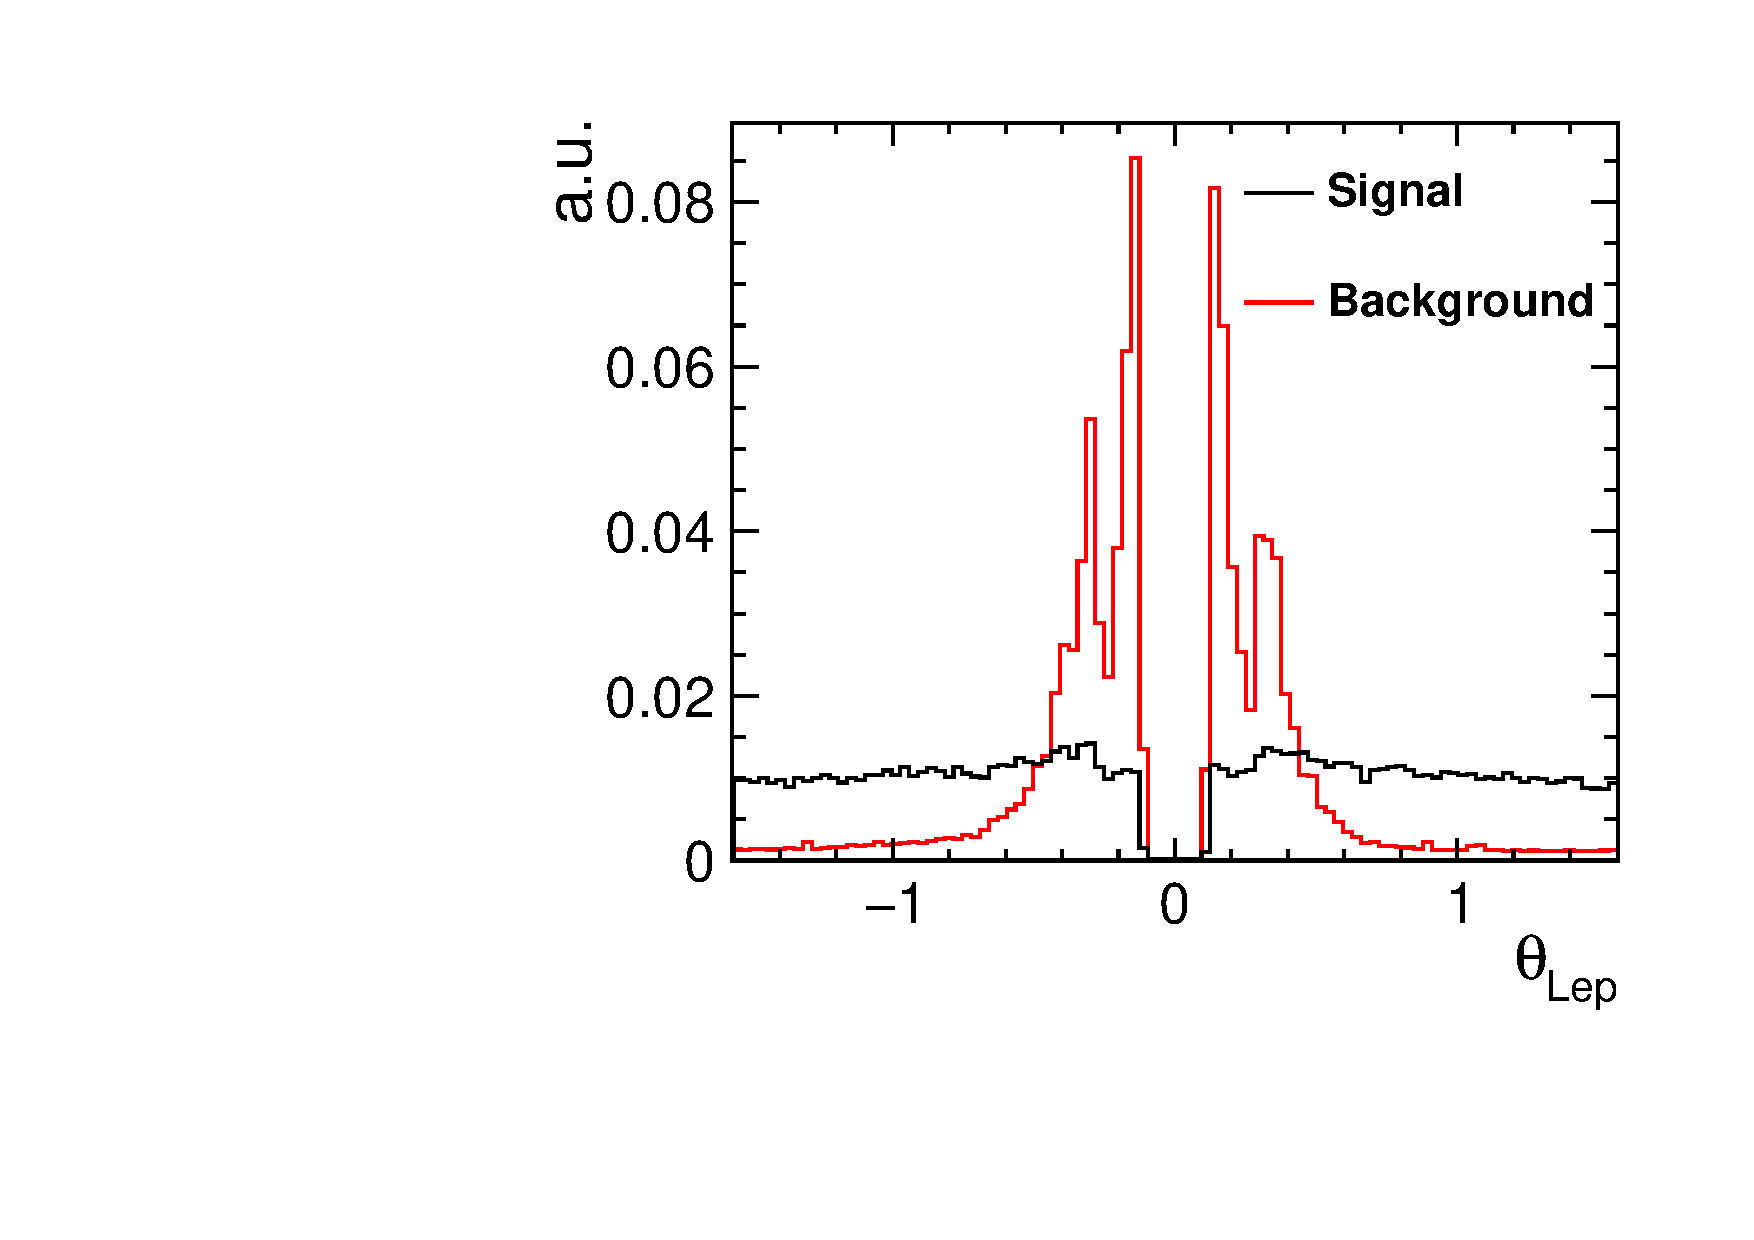
\includegraphics[width=0.75\linewidth]{Appendix/figures/DiraLep} 
    \caption{Angle of lepton relative to beam axis} 
    \vspace{4ex}
  \end{subfigure}%% 
  \begin{subfigure}[]{0.5\linewidth}
    \centering
    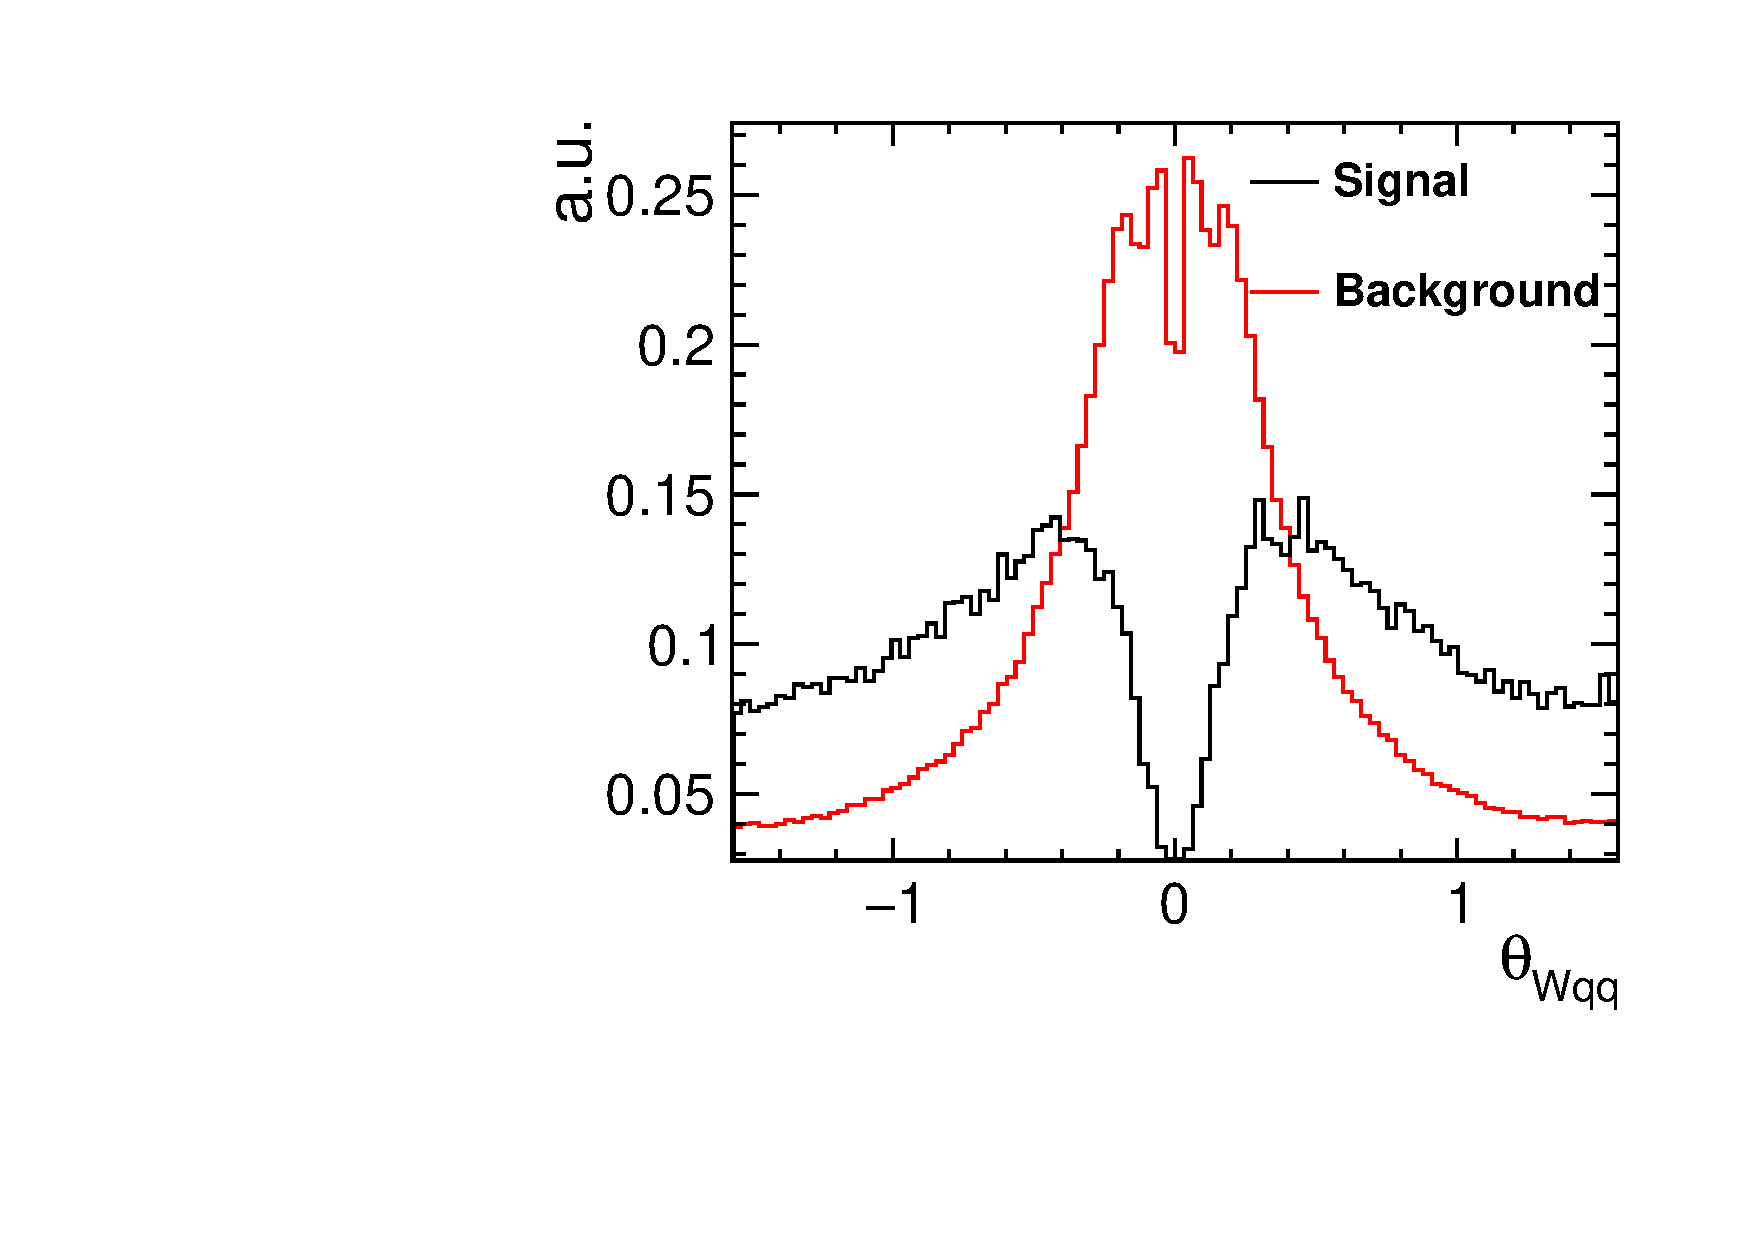
\includegraphics[width=0.75\linewidth]{Appendix/figures/DiraWqq} 
    \caption{Angle of W relative to beam axis} 
    \vspace{4ex}
  \end{subfigure}
    \begin{subfigure}[]{0.5\linewidth}
    \centering
    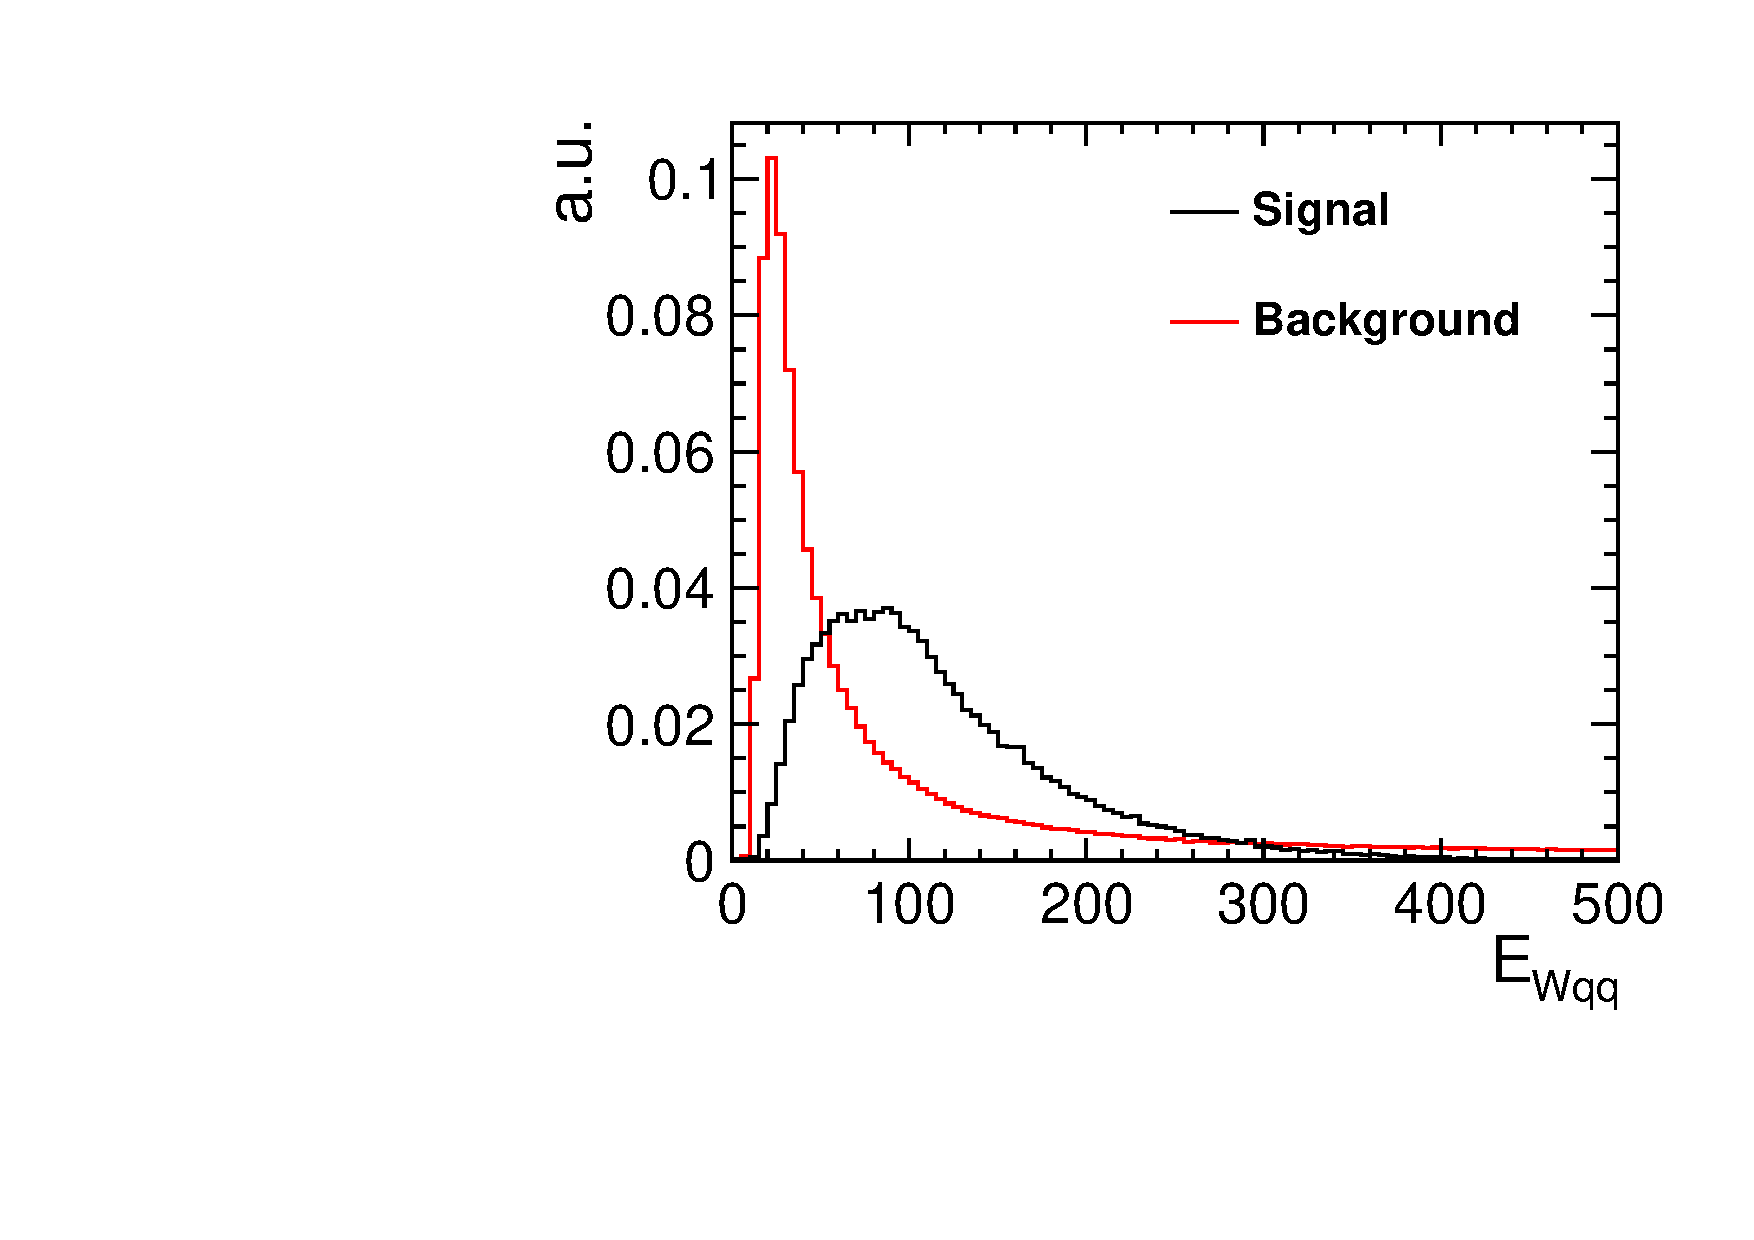
\includegraphics[width=0.75\linewidth]{Appendix/figures/EWqq} 
    \caption{Energy of hadronically decaying W} 
    \vspace{4ex}
  \end{subfigure}%% 
  \begin{subfigure}[]{0.5\linewidth}
    \centering
    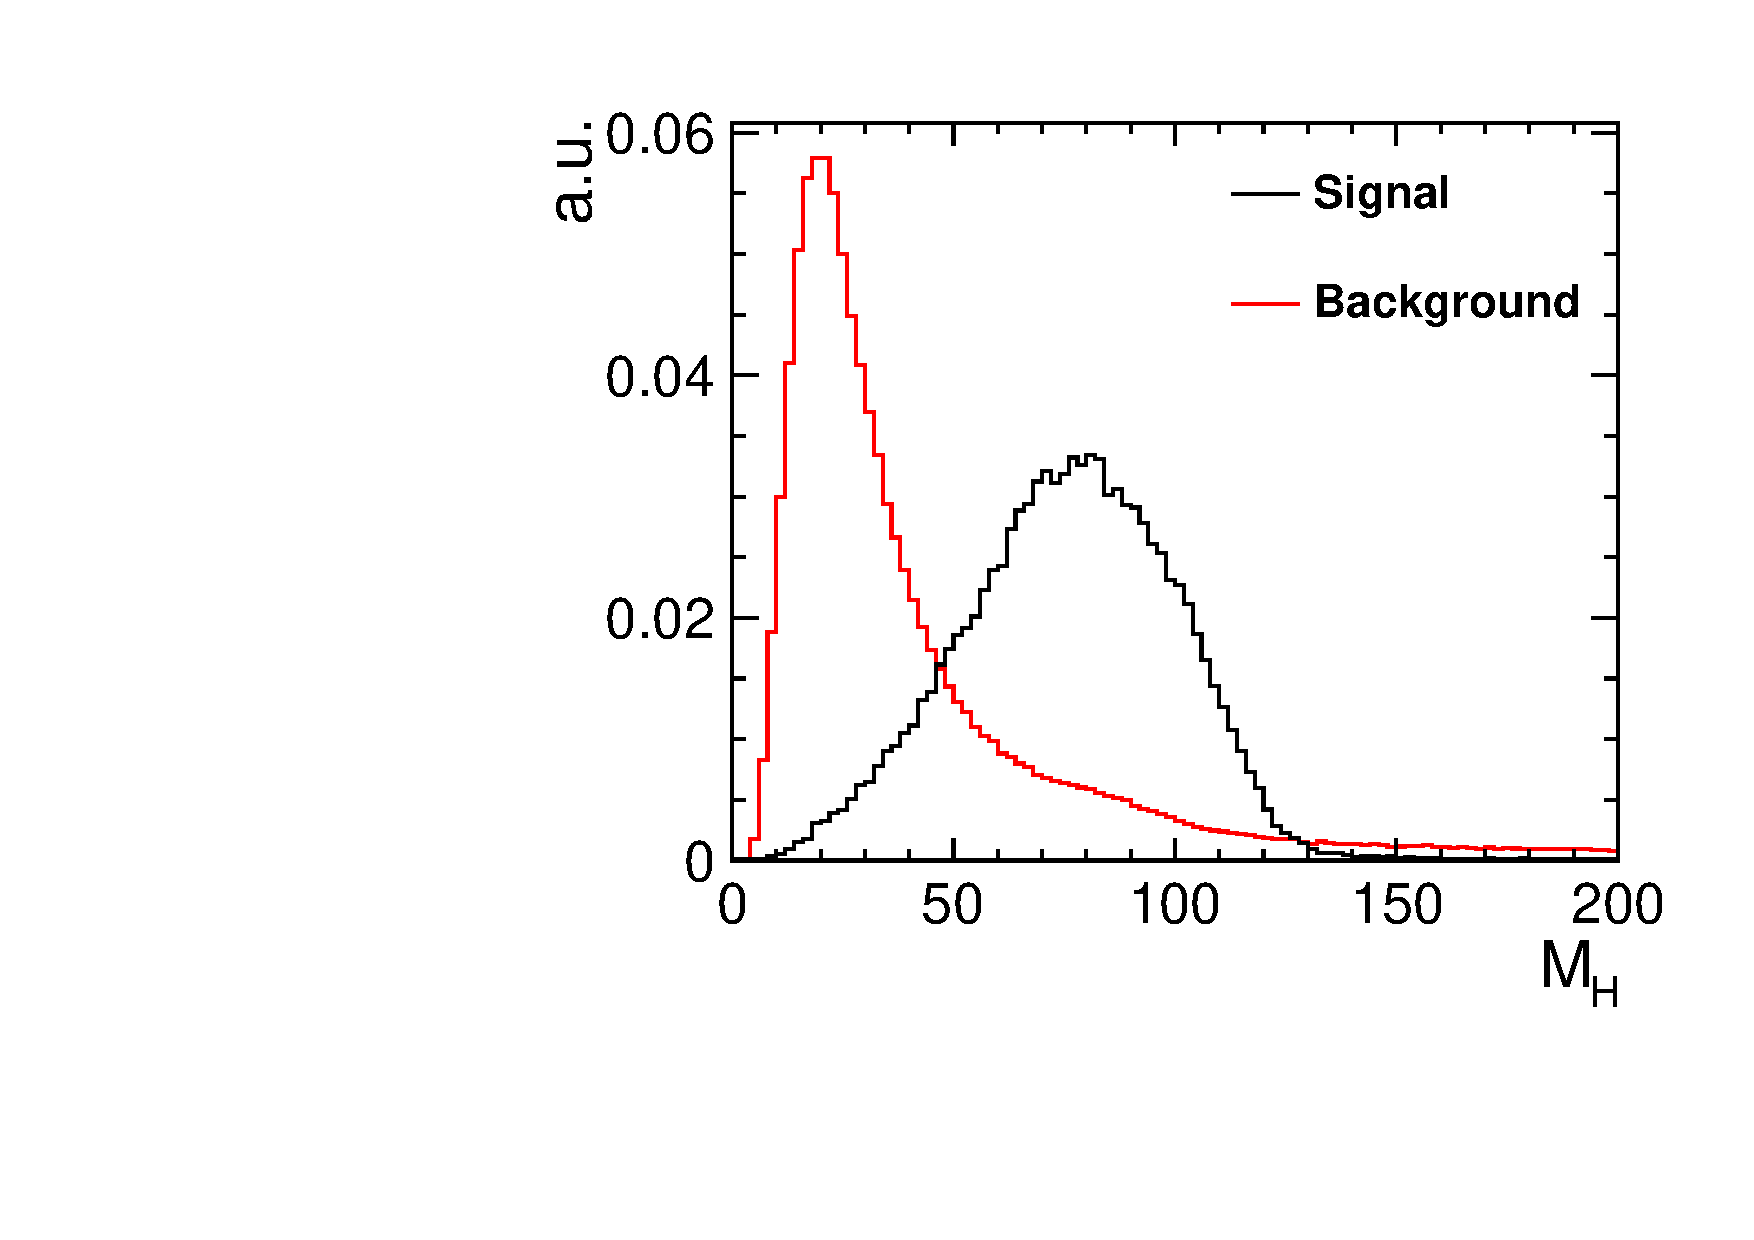
\includegraphics[width=0.75\linewidth]{Appendix/figures/HiggsMass} 
    \caption{Reconstructed Higgs mass} 
    \vspace{4ex}
  \end{subfigure}
    \begin{subfigure}[]{0.5\linewidth}
    \centering
    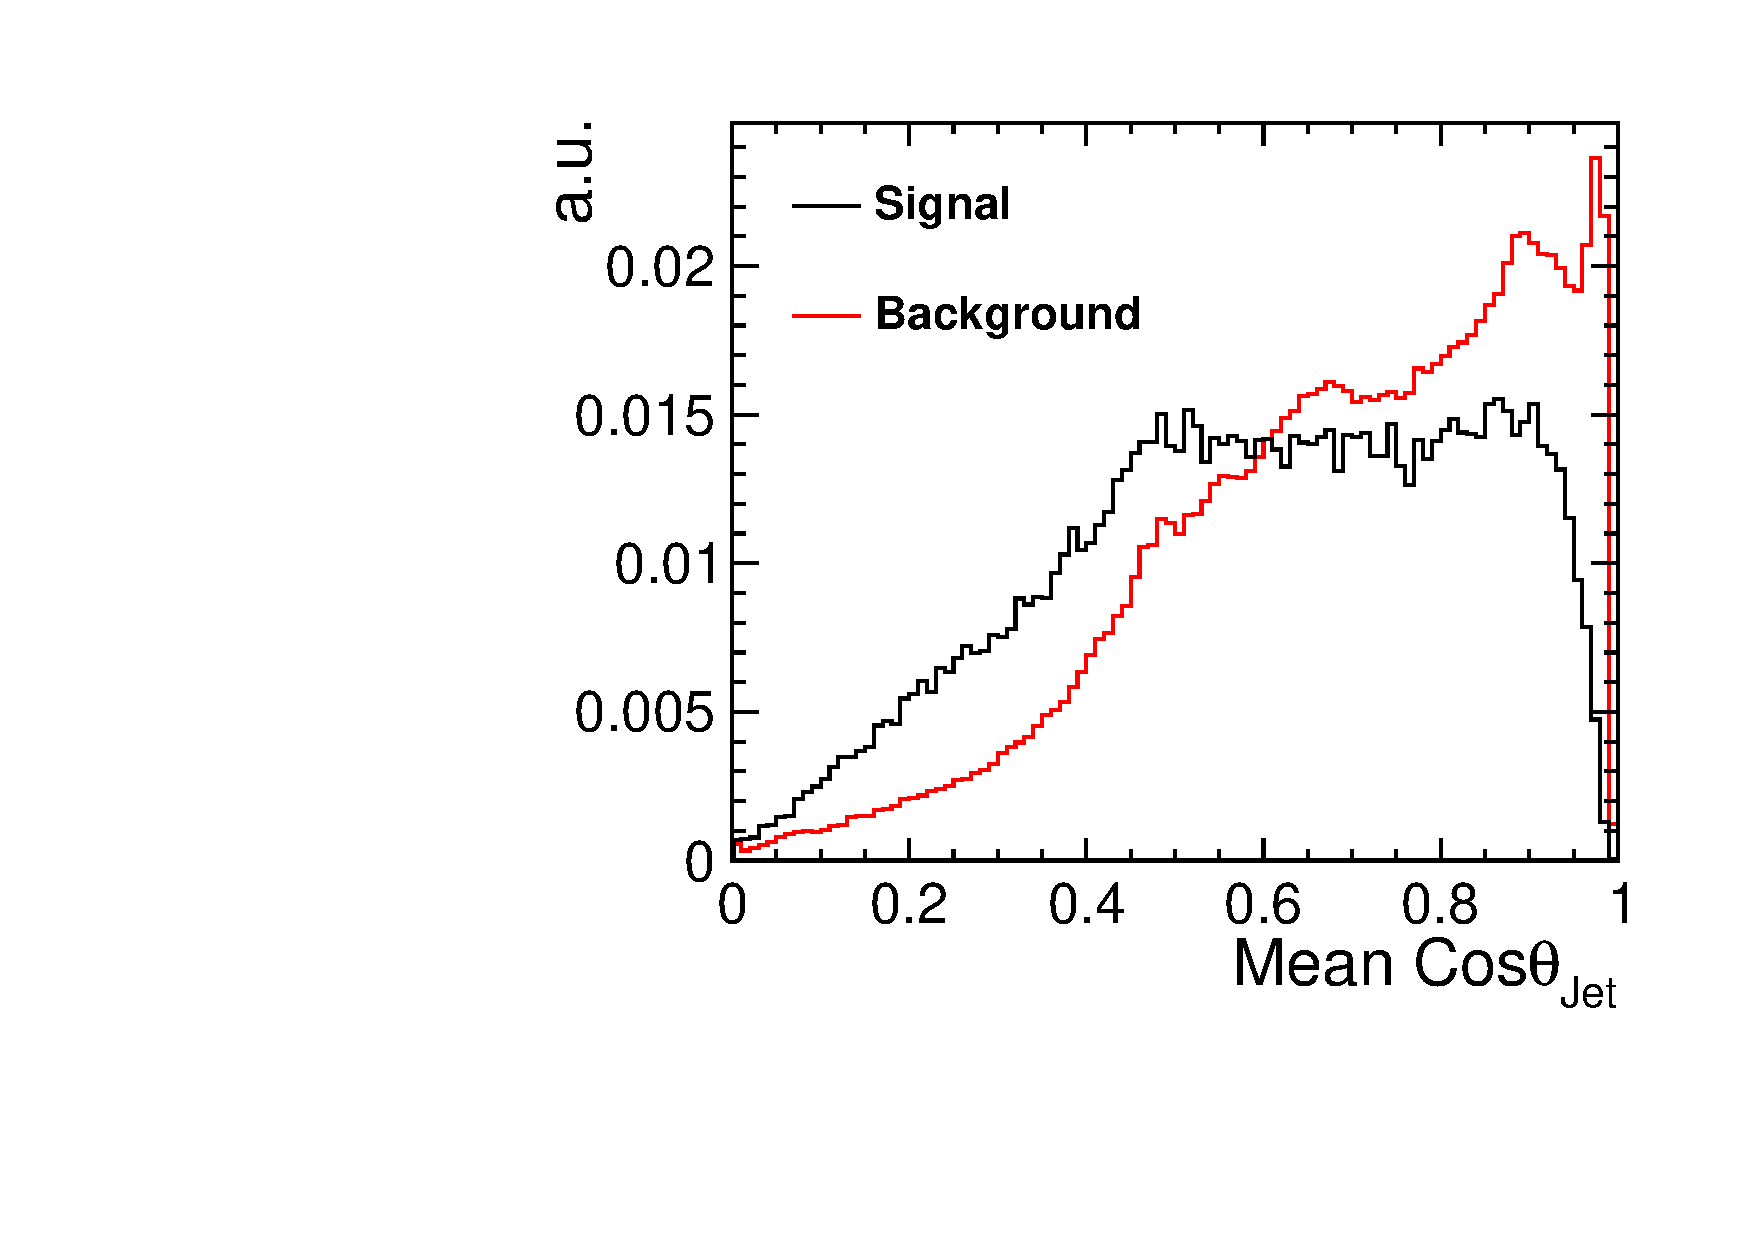
\includegraphics[width=0.75\linewidth]{Appendix/figures/JetCosTheta} 
    \caption{Average cos$\theta$ of jets} 
  \end{subfigure}%%
  \begin{subfigure}[]{0.5\linewidth}
    \centering
    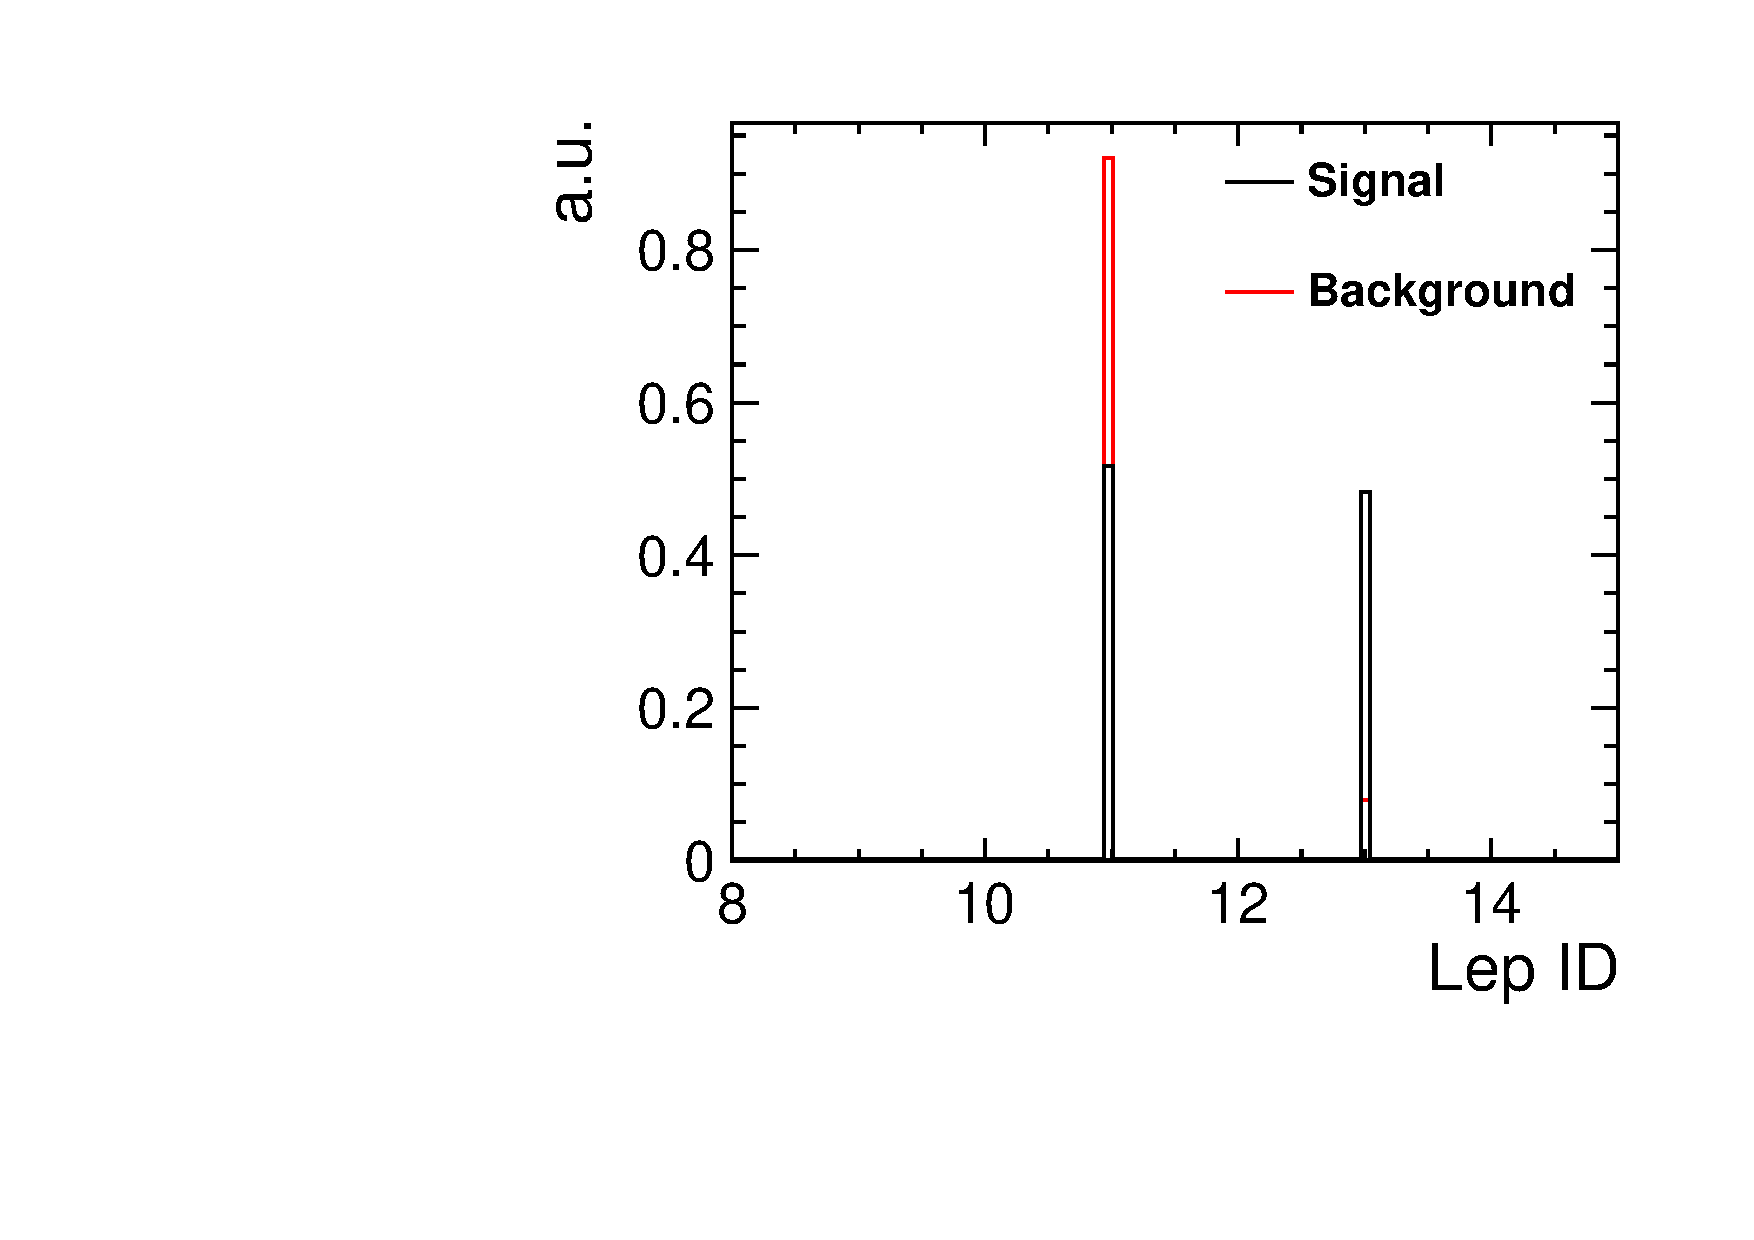
\includegraphics[width=0.75\linewidth]{Appendix/figures/LepID} 
    \caption{Lepton PID} 
  \end{subfigure}
\end{figure}


\begin{figure}[]\ContinuedFloat
    \begin{subfigure}[]{0.5\linewidth}
    \centering
    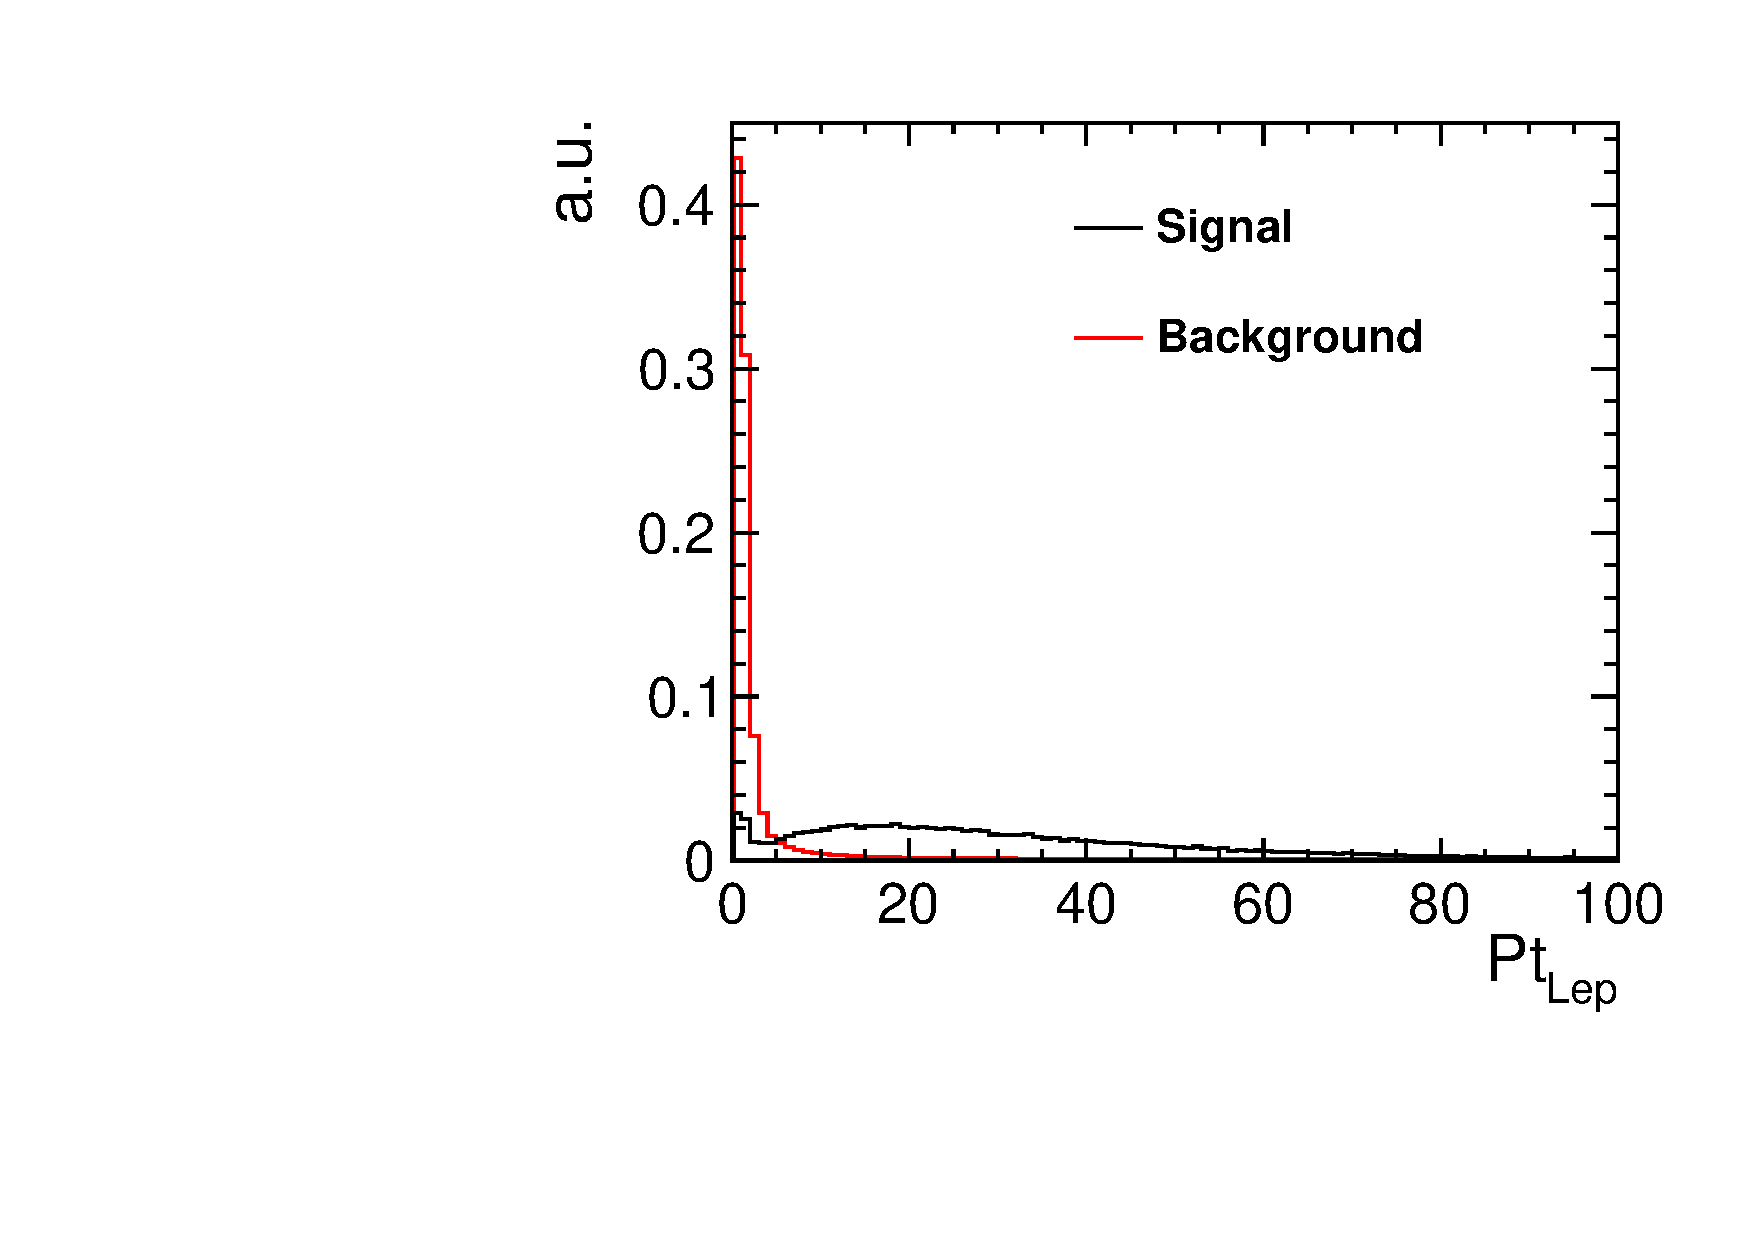
\includegraphics[width=0.75\linewidth]{Appendix/figures/LepPt} 
    \caption{Lepton Pt} 
  \end{subfigure}%%
  \begin{subfigure}[]{0.5\linewidth}
    \centering
    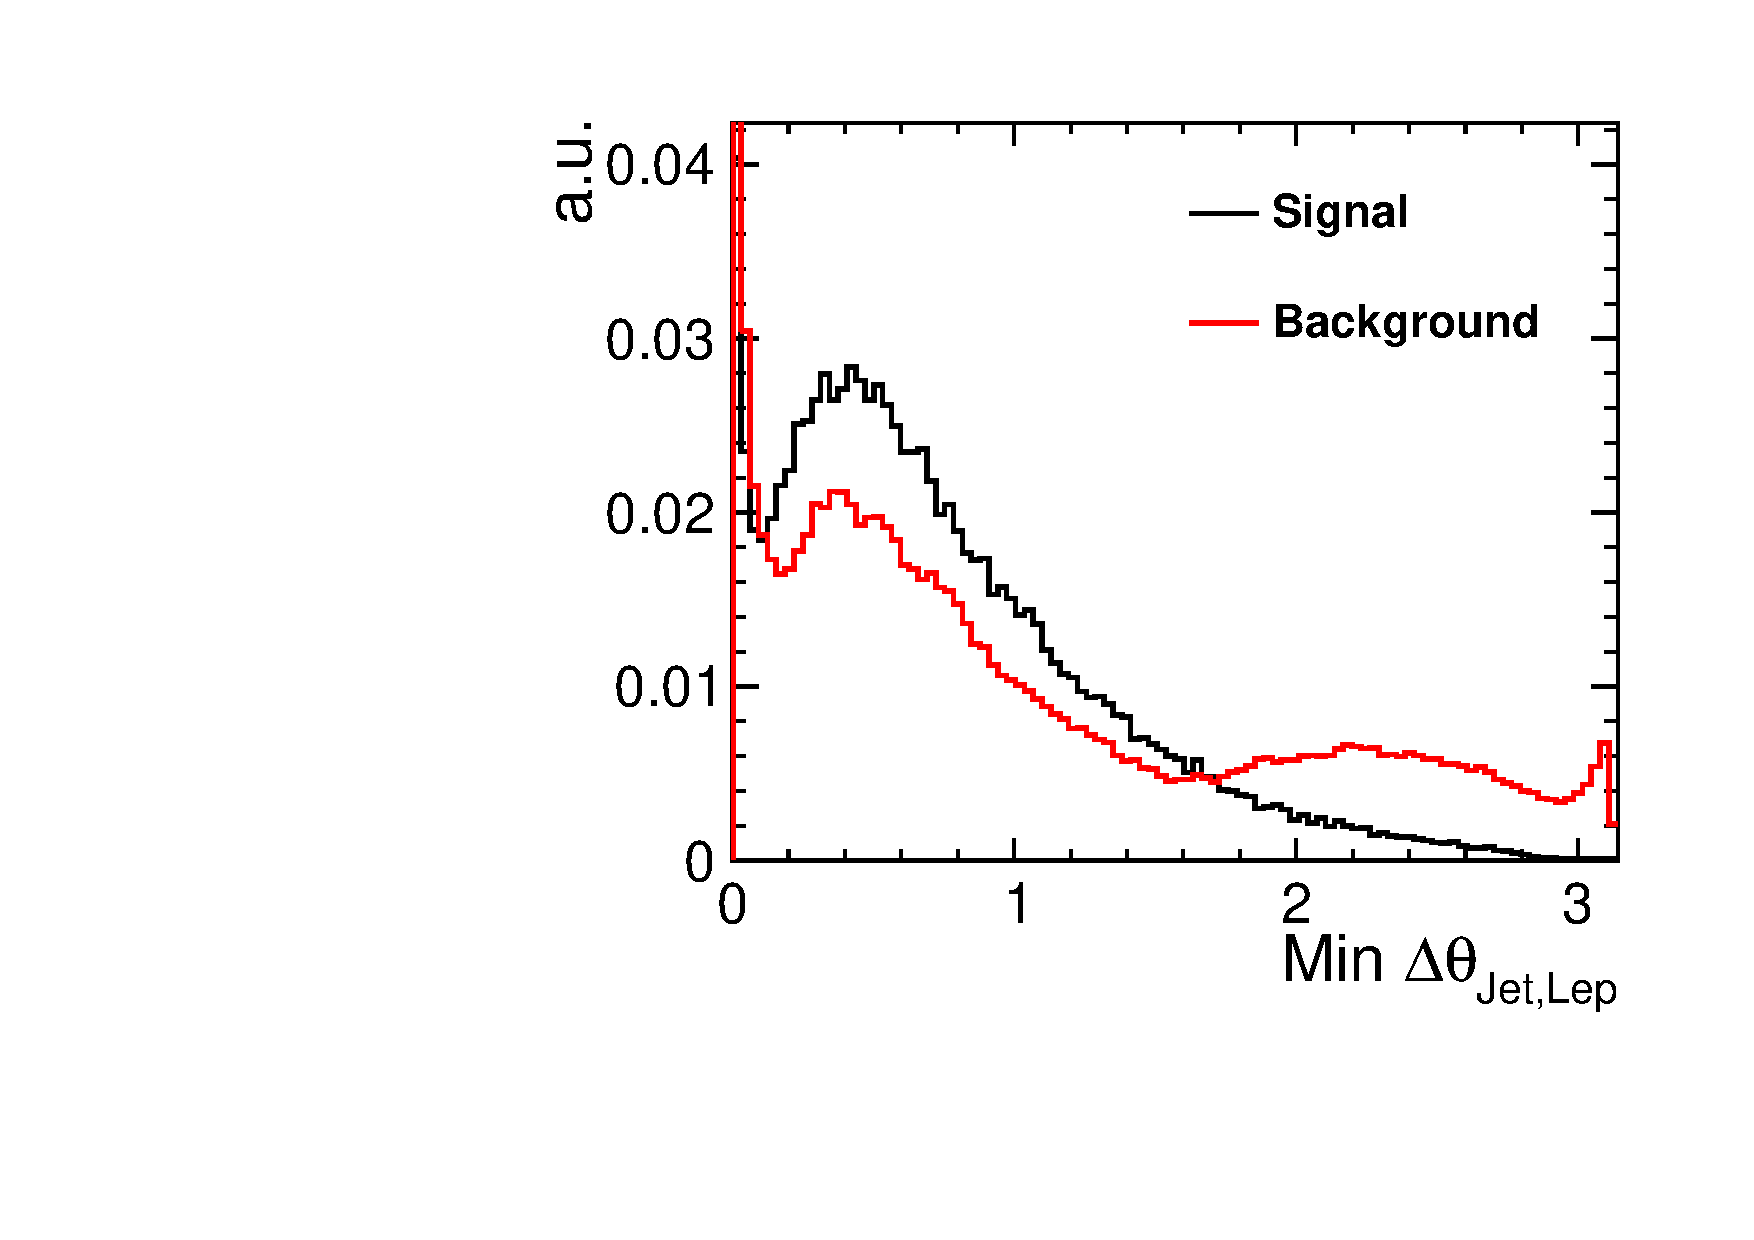
\includegraphics[width=0.75\linewidth]{Appendix/figures/MinJetLepAngSep} 
    \caption{Angular separation between lepton and nearest jet} 
  \end{subfigure}
  \begin{subfigure}[]{0.5\linewidth}
    \centering
    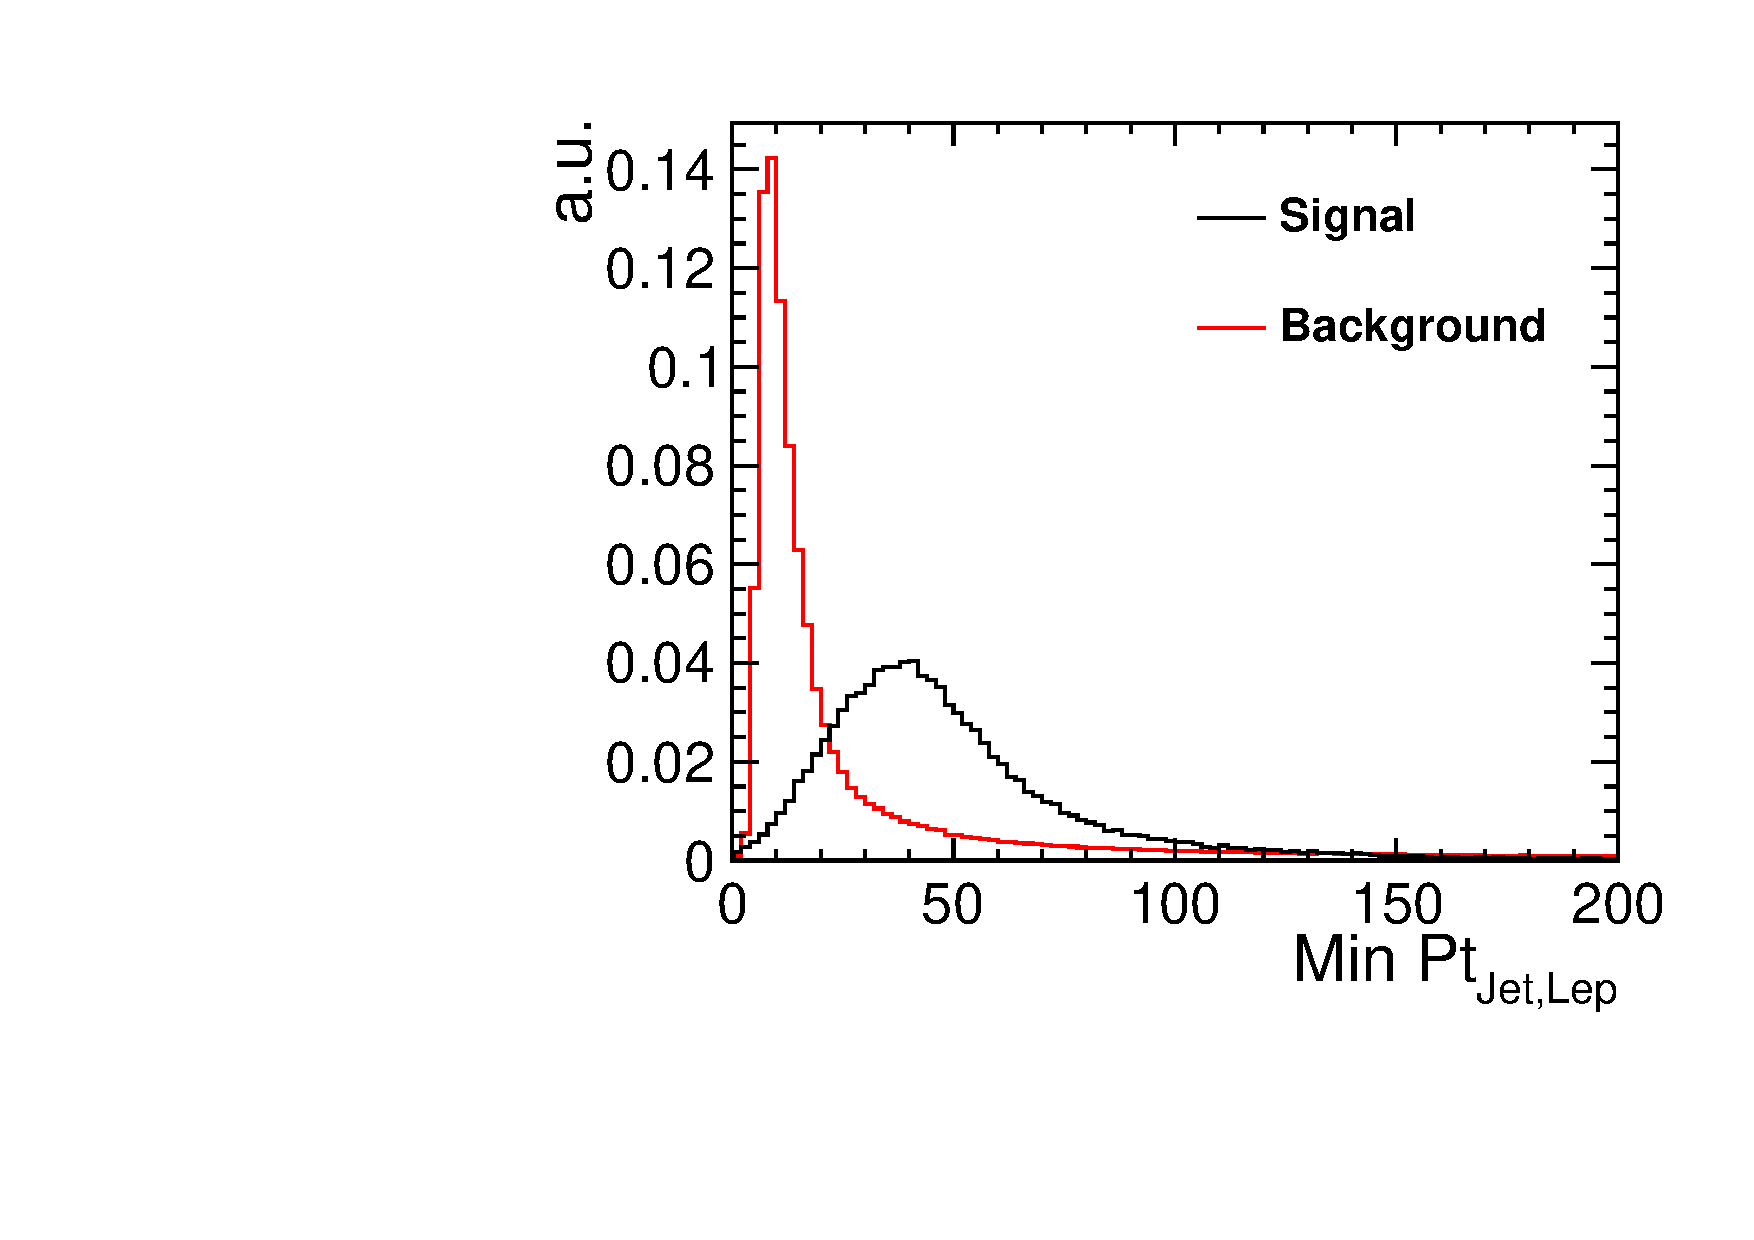
\includegraphics[width=0.75\linewidth]{Appendix/figures/MinJetLepPt} 
    \caption{Relative Pt between lepton and nearest jet} 
    \vspace{4ex}
  \end{subfigure}%% 
  \begin{subfigure}[]{0.5\linewidth}
    \centering
    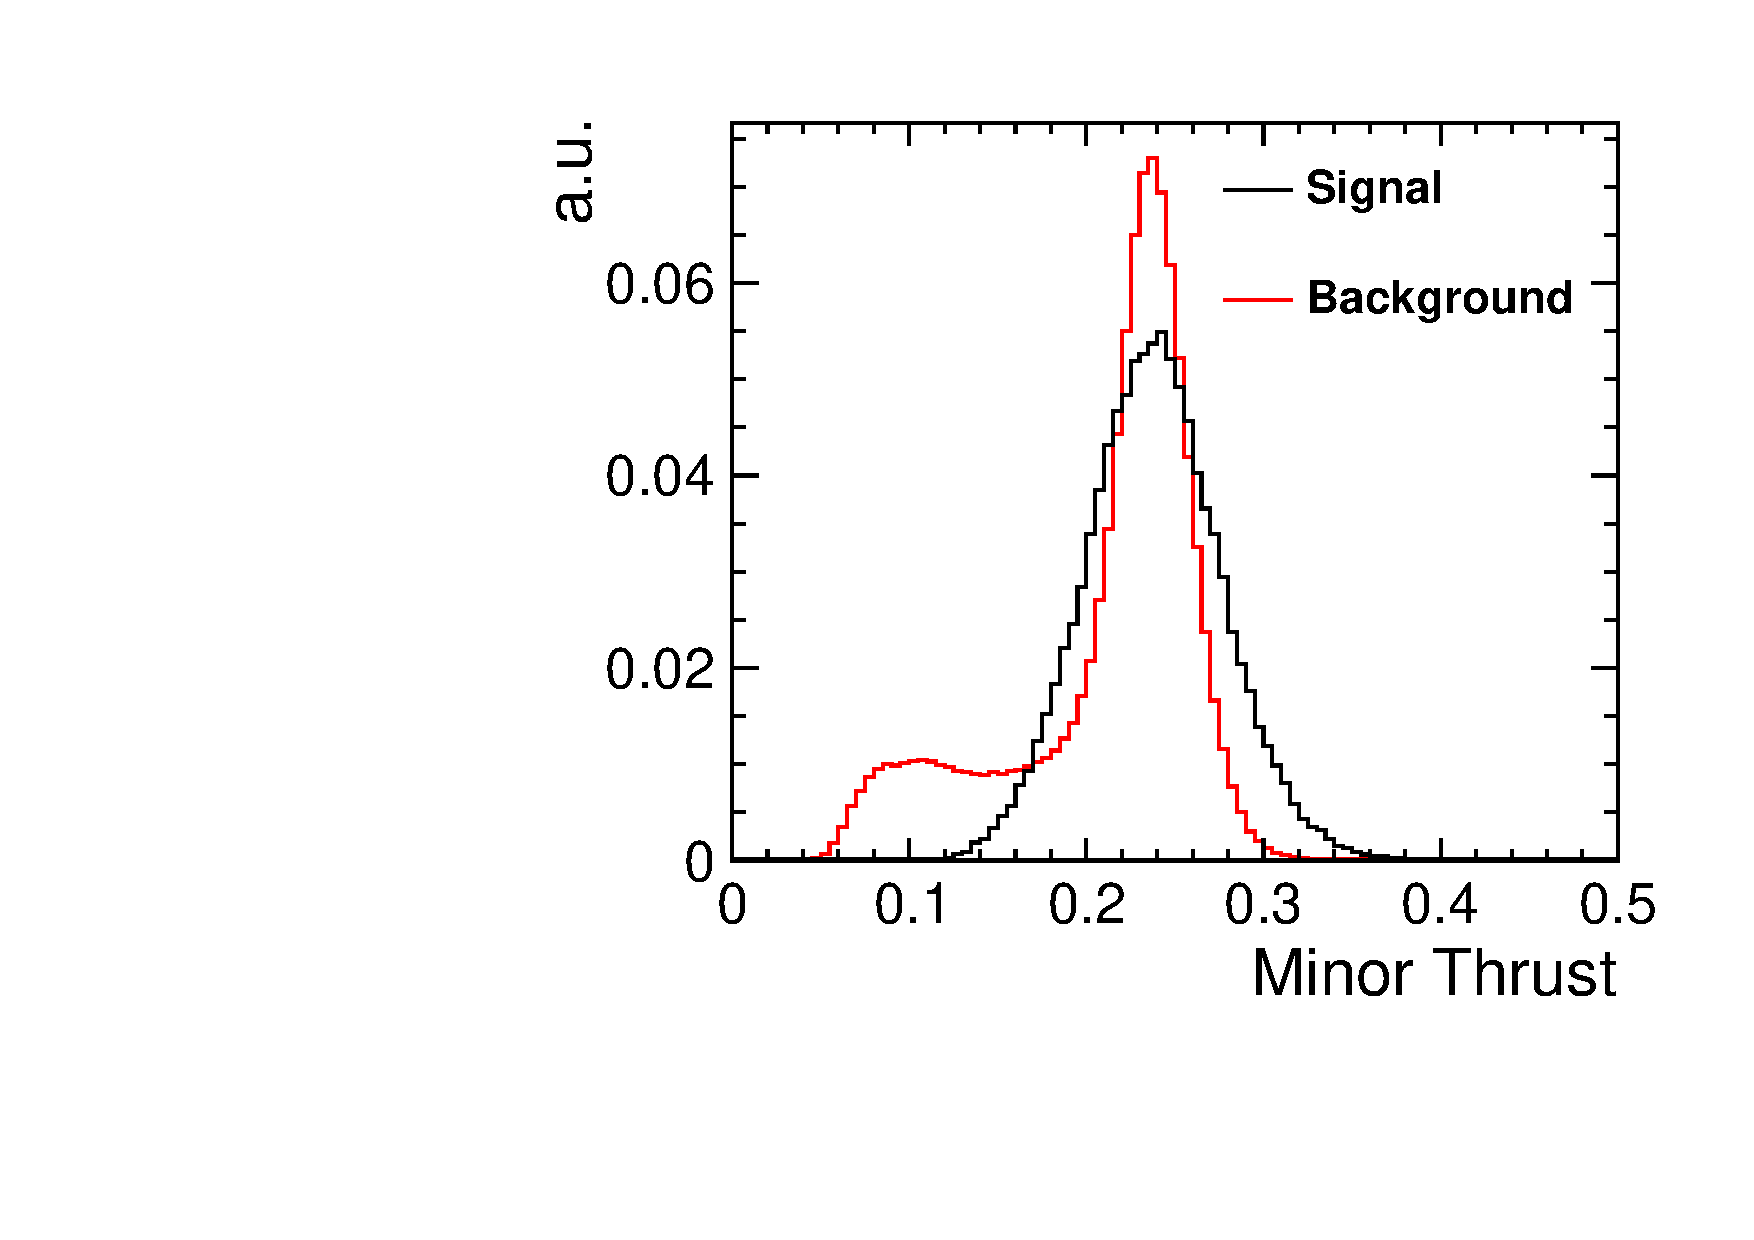
\includegraphics[width=0.75\linewidth]{Appendix/figures/MinorThrust} 
    \caption{Minor Thrust of the event} 
    \vspace{4ex}
  \end{subfigure} 
  \begin{subfigure}[]{0.5\linewidth}
    \centering
    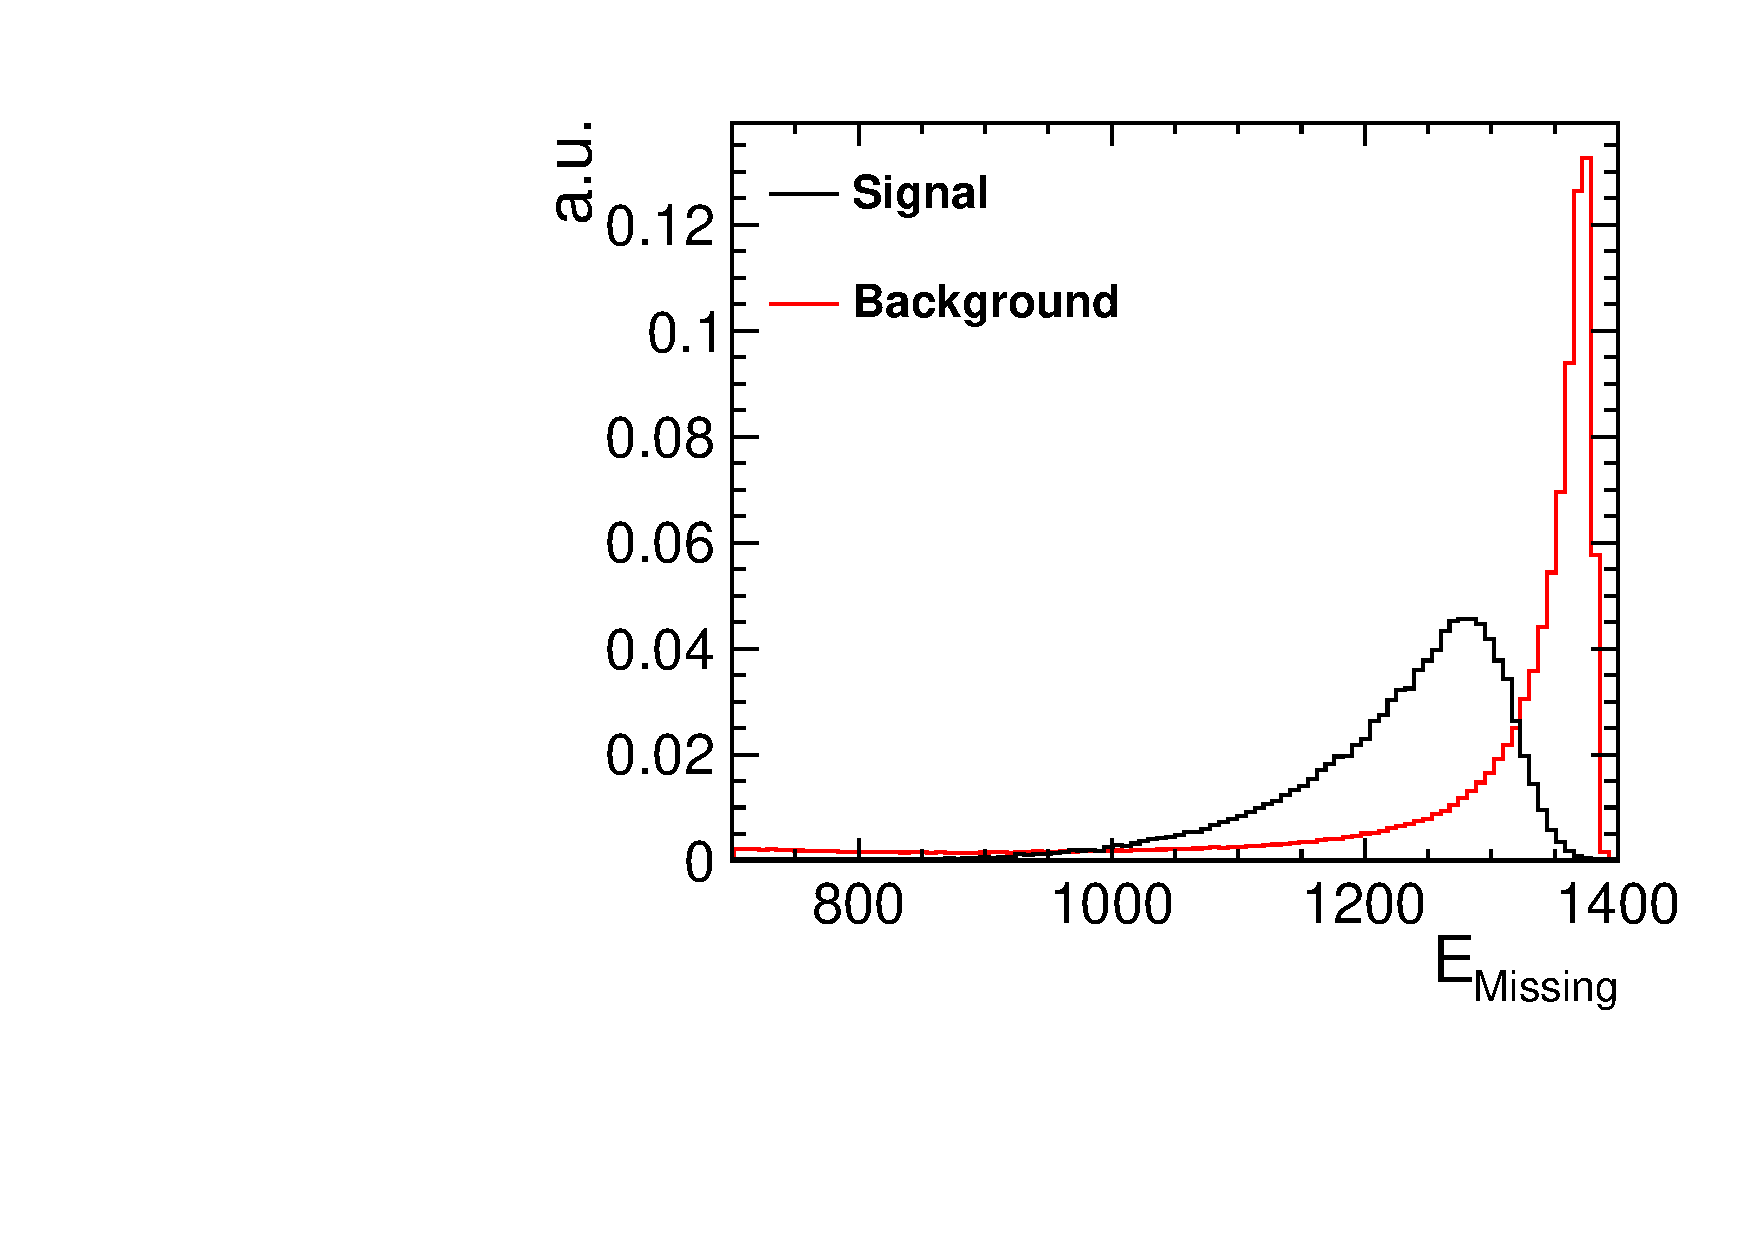
\includegraphics[width=0.75\linewidth]{Appendix/figures/MissingE} 
    \caption{Missing energy} 
    \vspace{4ex}
  \end{subfigure}%%
  \begin{subfigure}[]{0.5\linewidth}
    \centering
    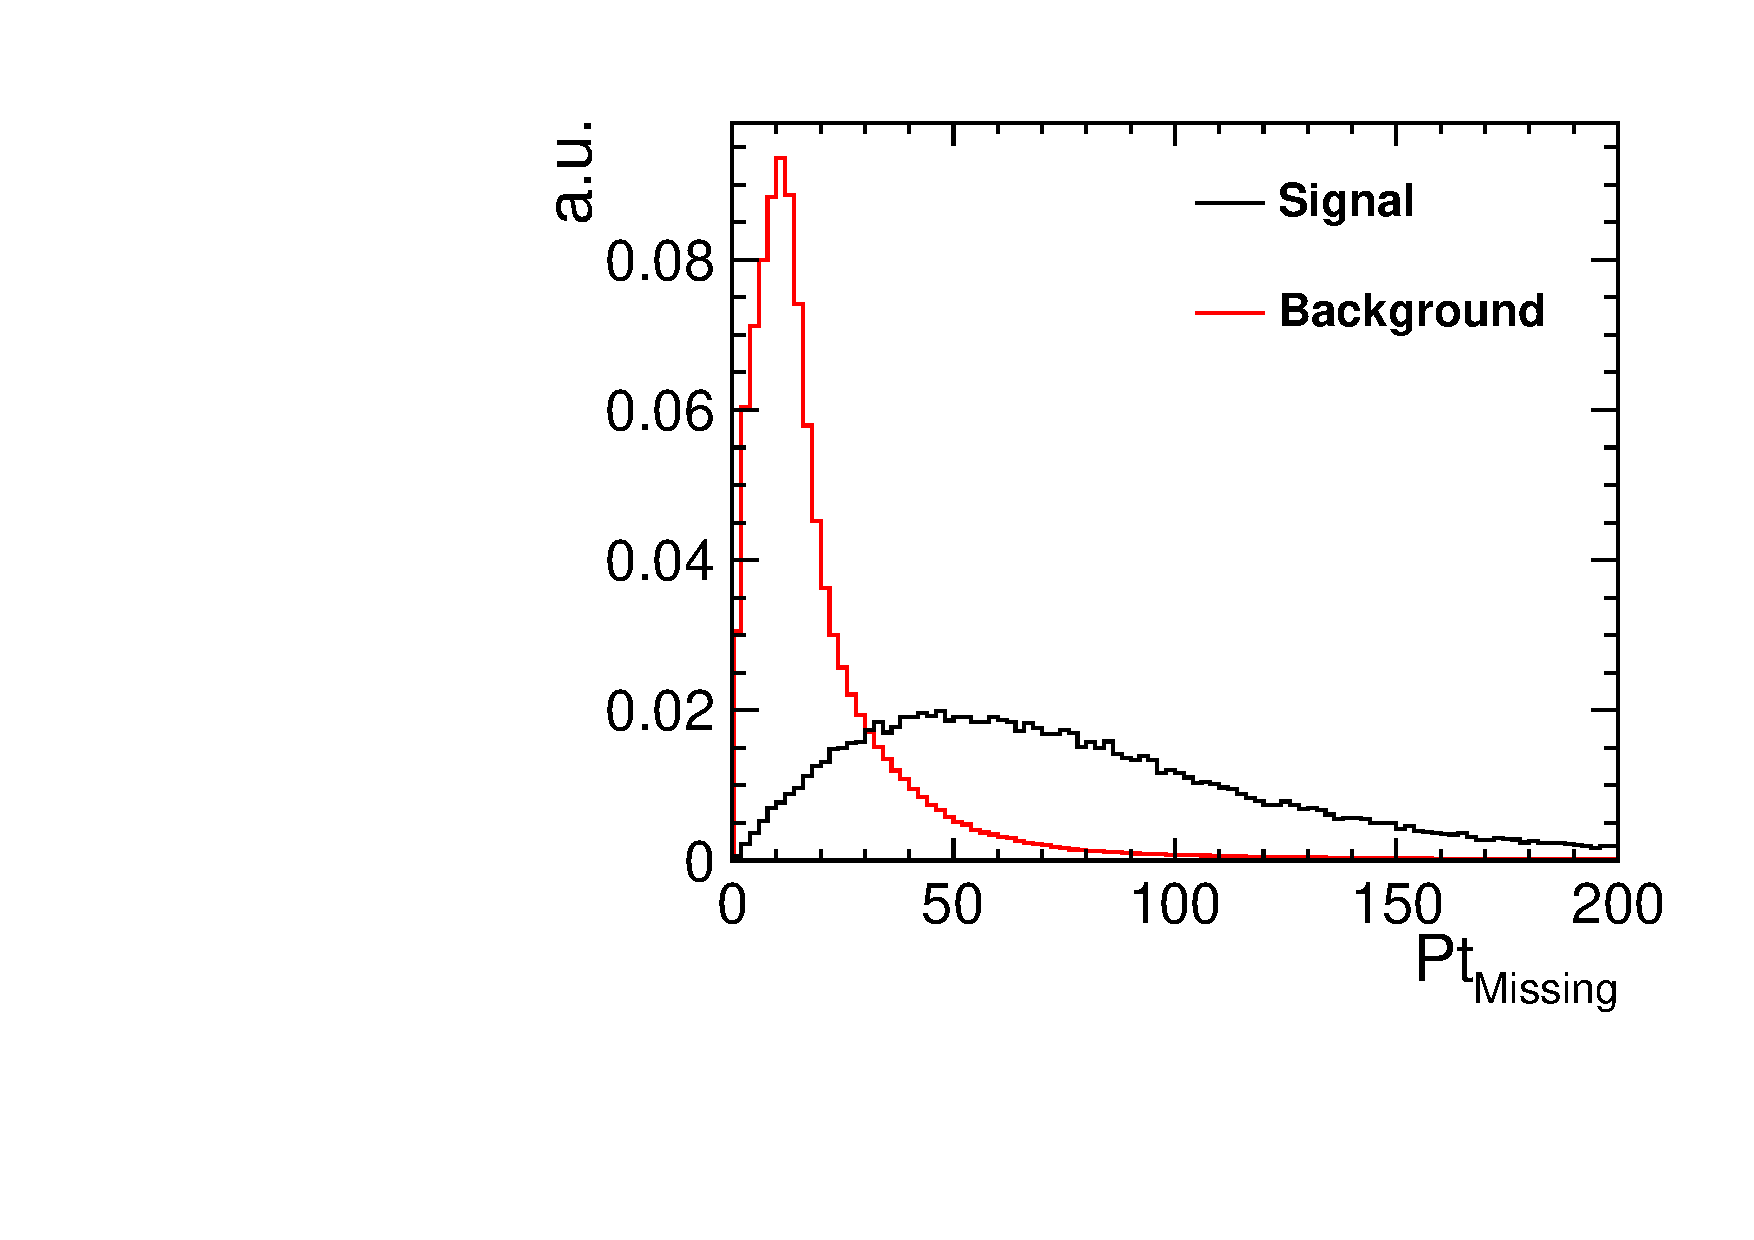
\includegraphics[width=0.75\linewidth]{Appendix/figures/MissingPt} 
    \caption{Missing transverse momentum} 
    \vspace{4ex}
  \end{subfigure}
\end{figure}

\begin{figure}[]\ContinuedFloat 
   \begin{subfigure}[]{0.5\linewidth}
    \centering
    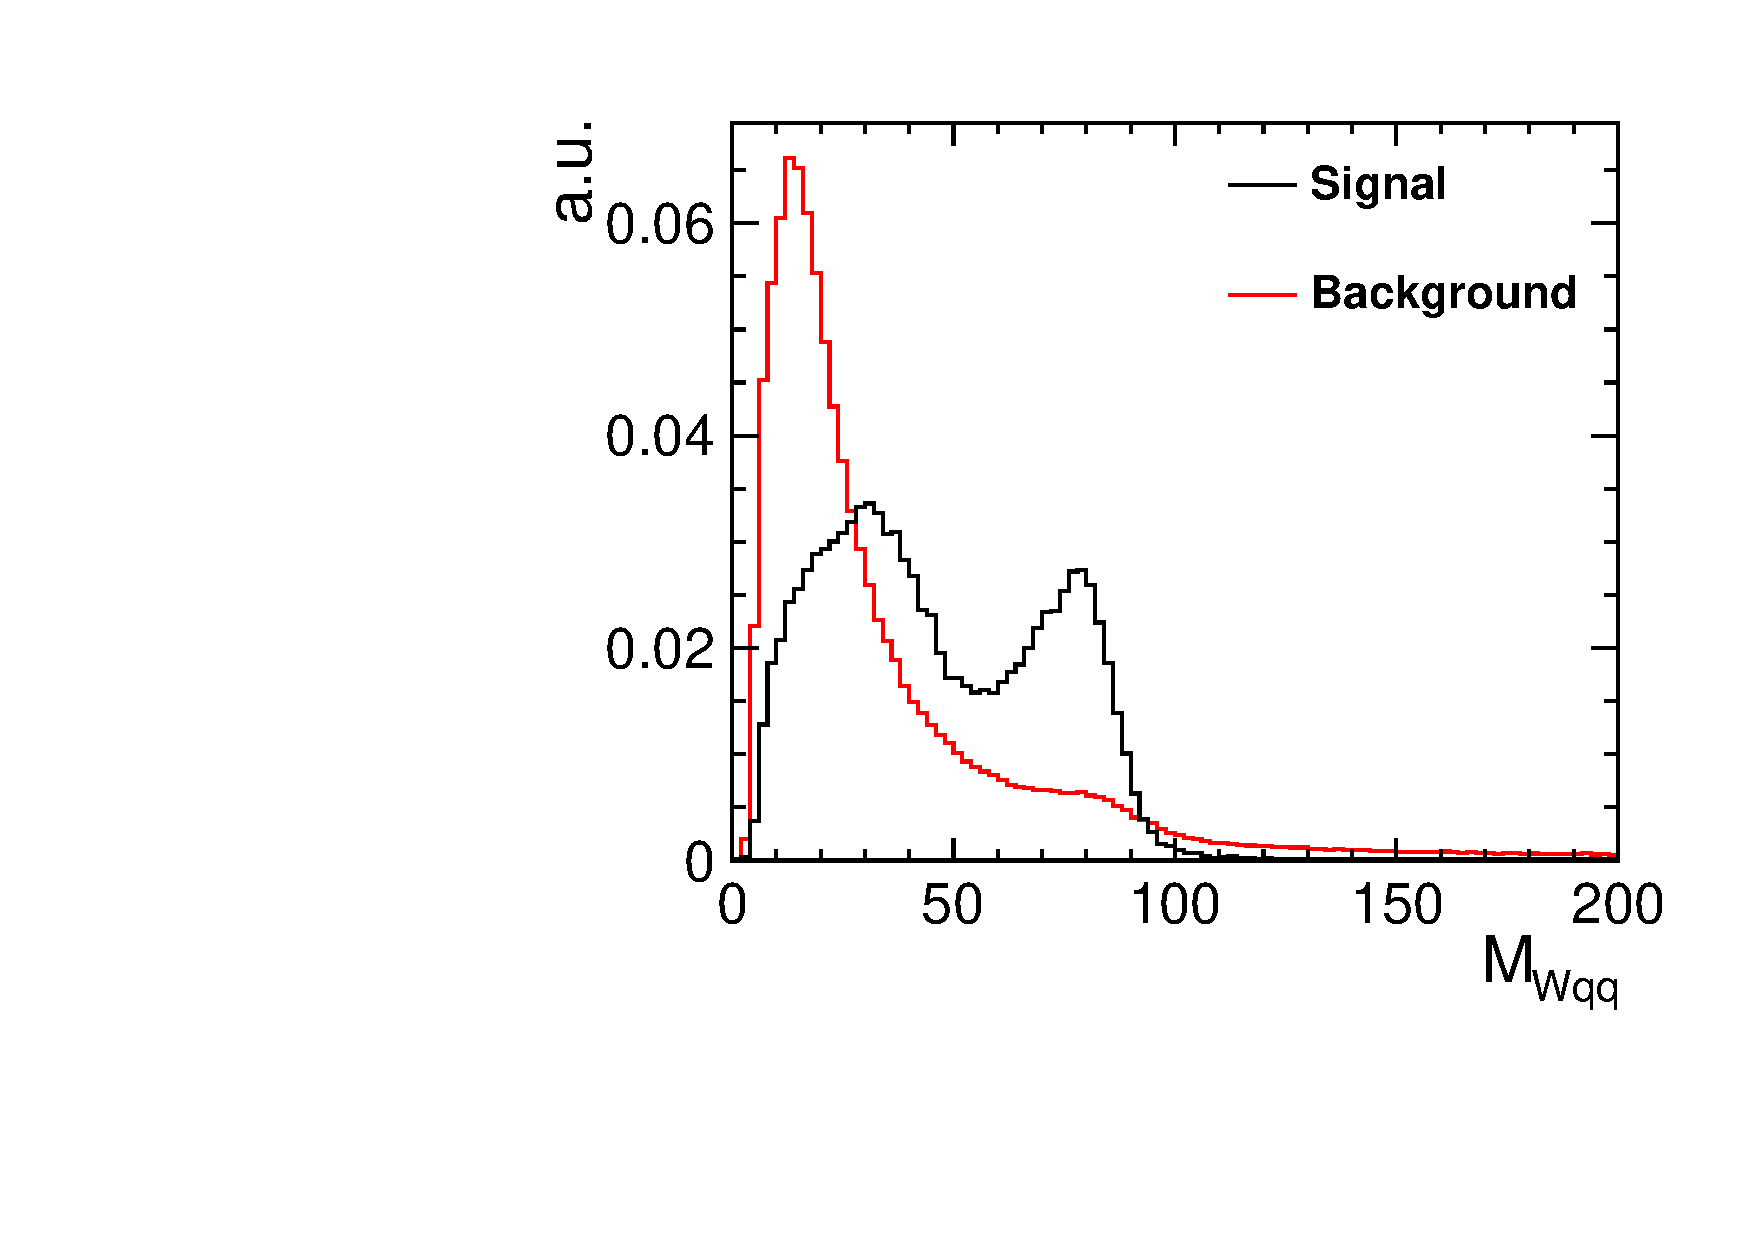
\includegraphics[width=0.75\linewidth]{Appendix/figures/MWqq} 
    \caption{Mass of hadronically decaying W} 
    \vspace{4ex}
  \end{subfigure}%%
  \begin{subfigure}[]{0.5\linewidth}
    \centering
    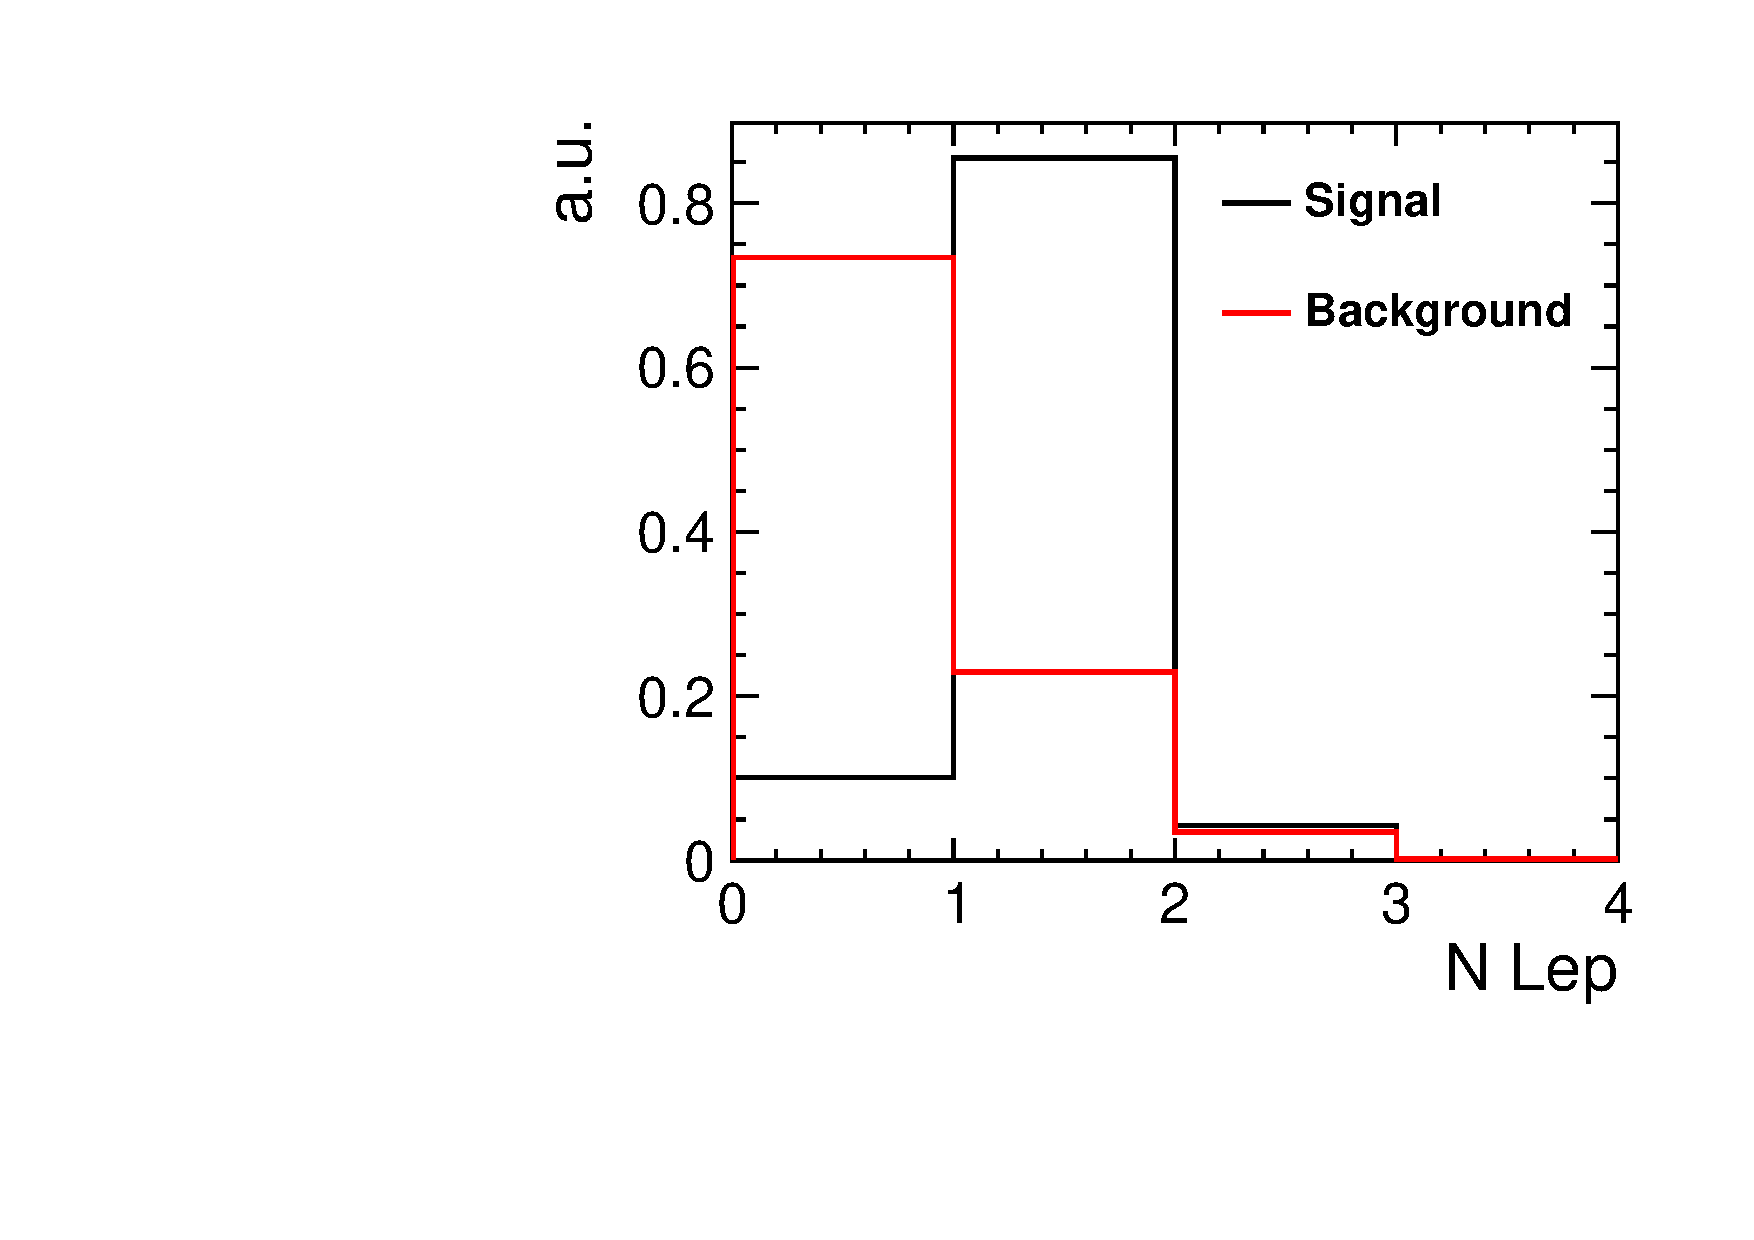
\includegraphics[width=0.75\linewidth]{Appendix/figures/nLep} 
    \caption{Number of reconstructed leptons} 
    \vspace{4ex}
  \end{subfigure}
  \begin{subfigure}[]{0.5\linewidth}
    \centering
    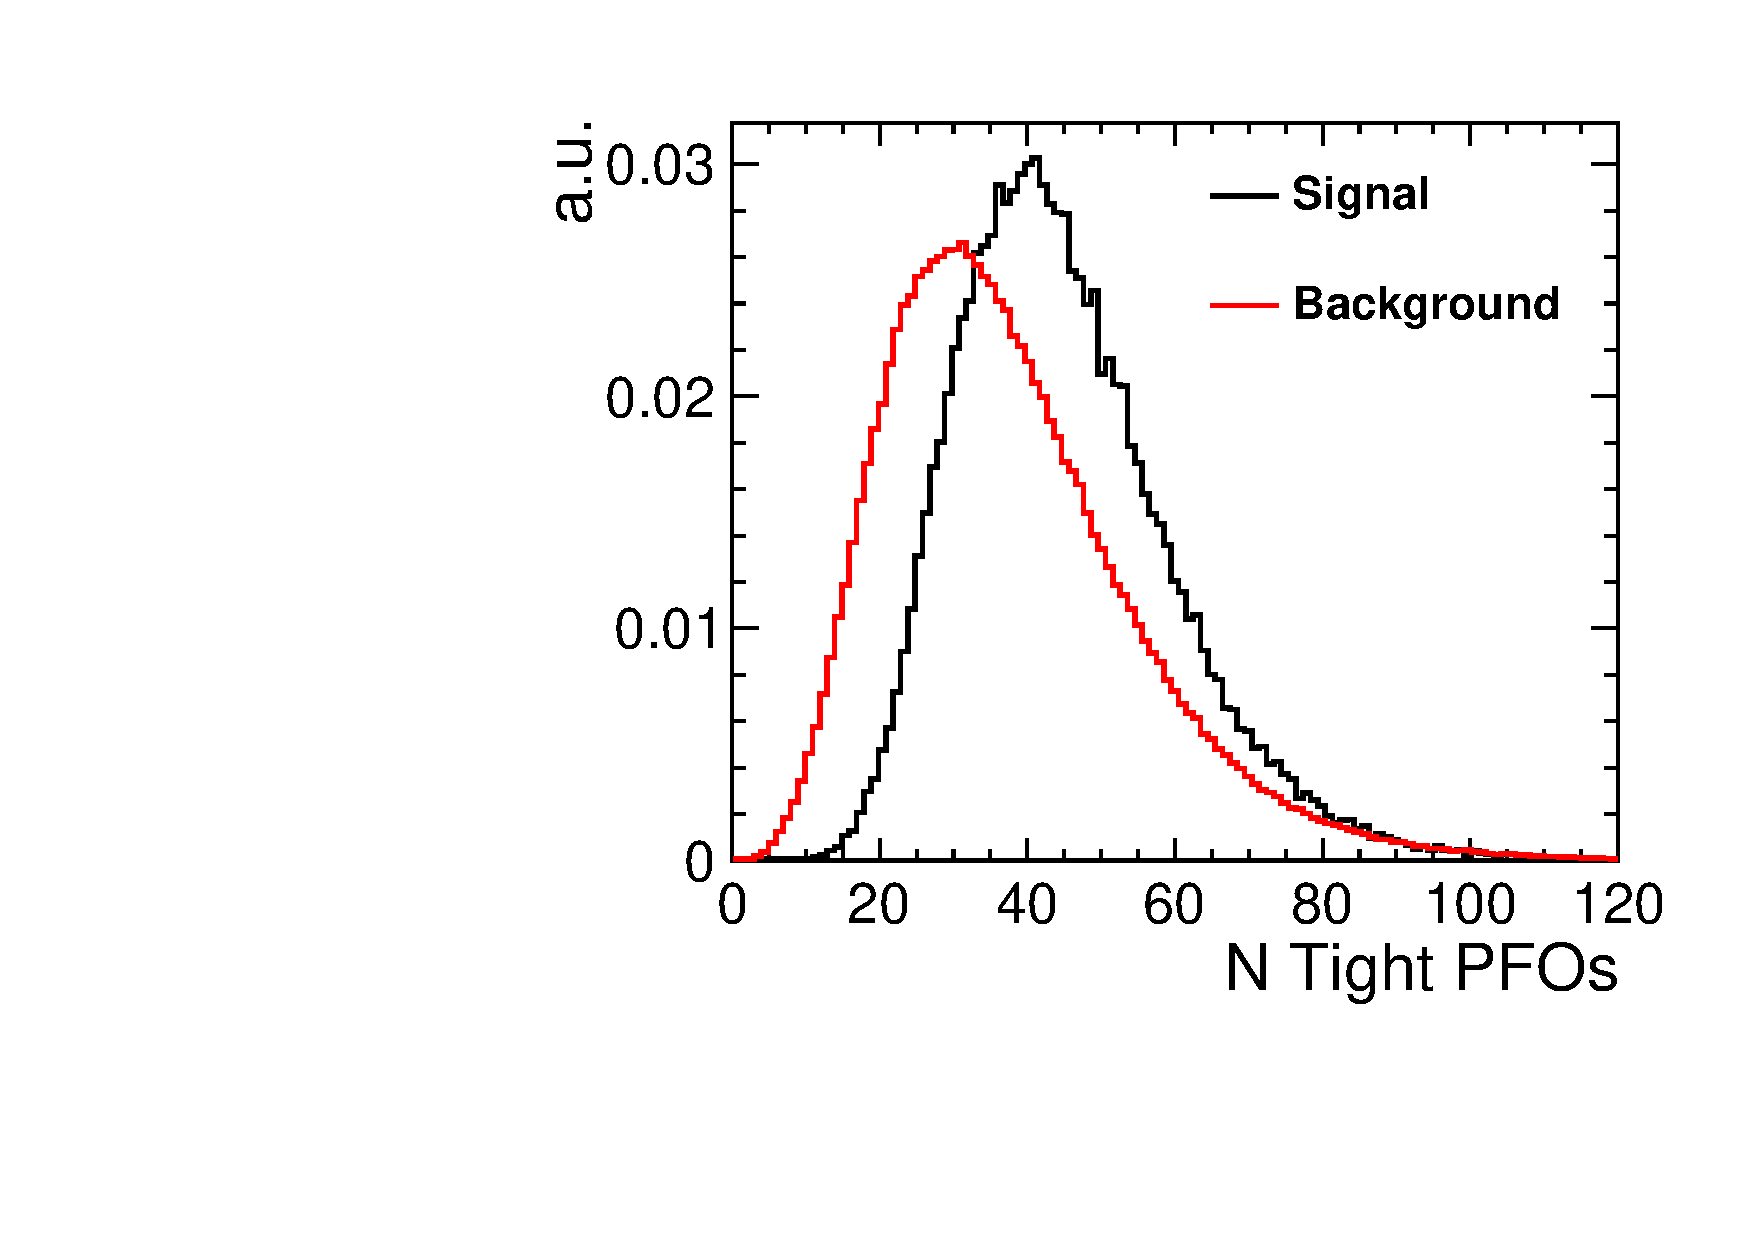
\includegraphics[width=0.75\linewidth]{Appendix/figures/NTightPFOs} 
    \caption{nPFOs passing tight timing cuts} 
    \vspace{4ex}
  \end{subfigure}%% 
  \begin{subfigure}[]{0.5\linewidth}
    \centering
    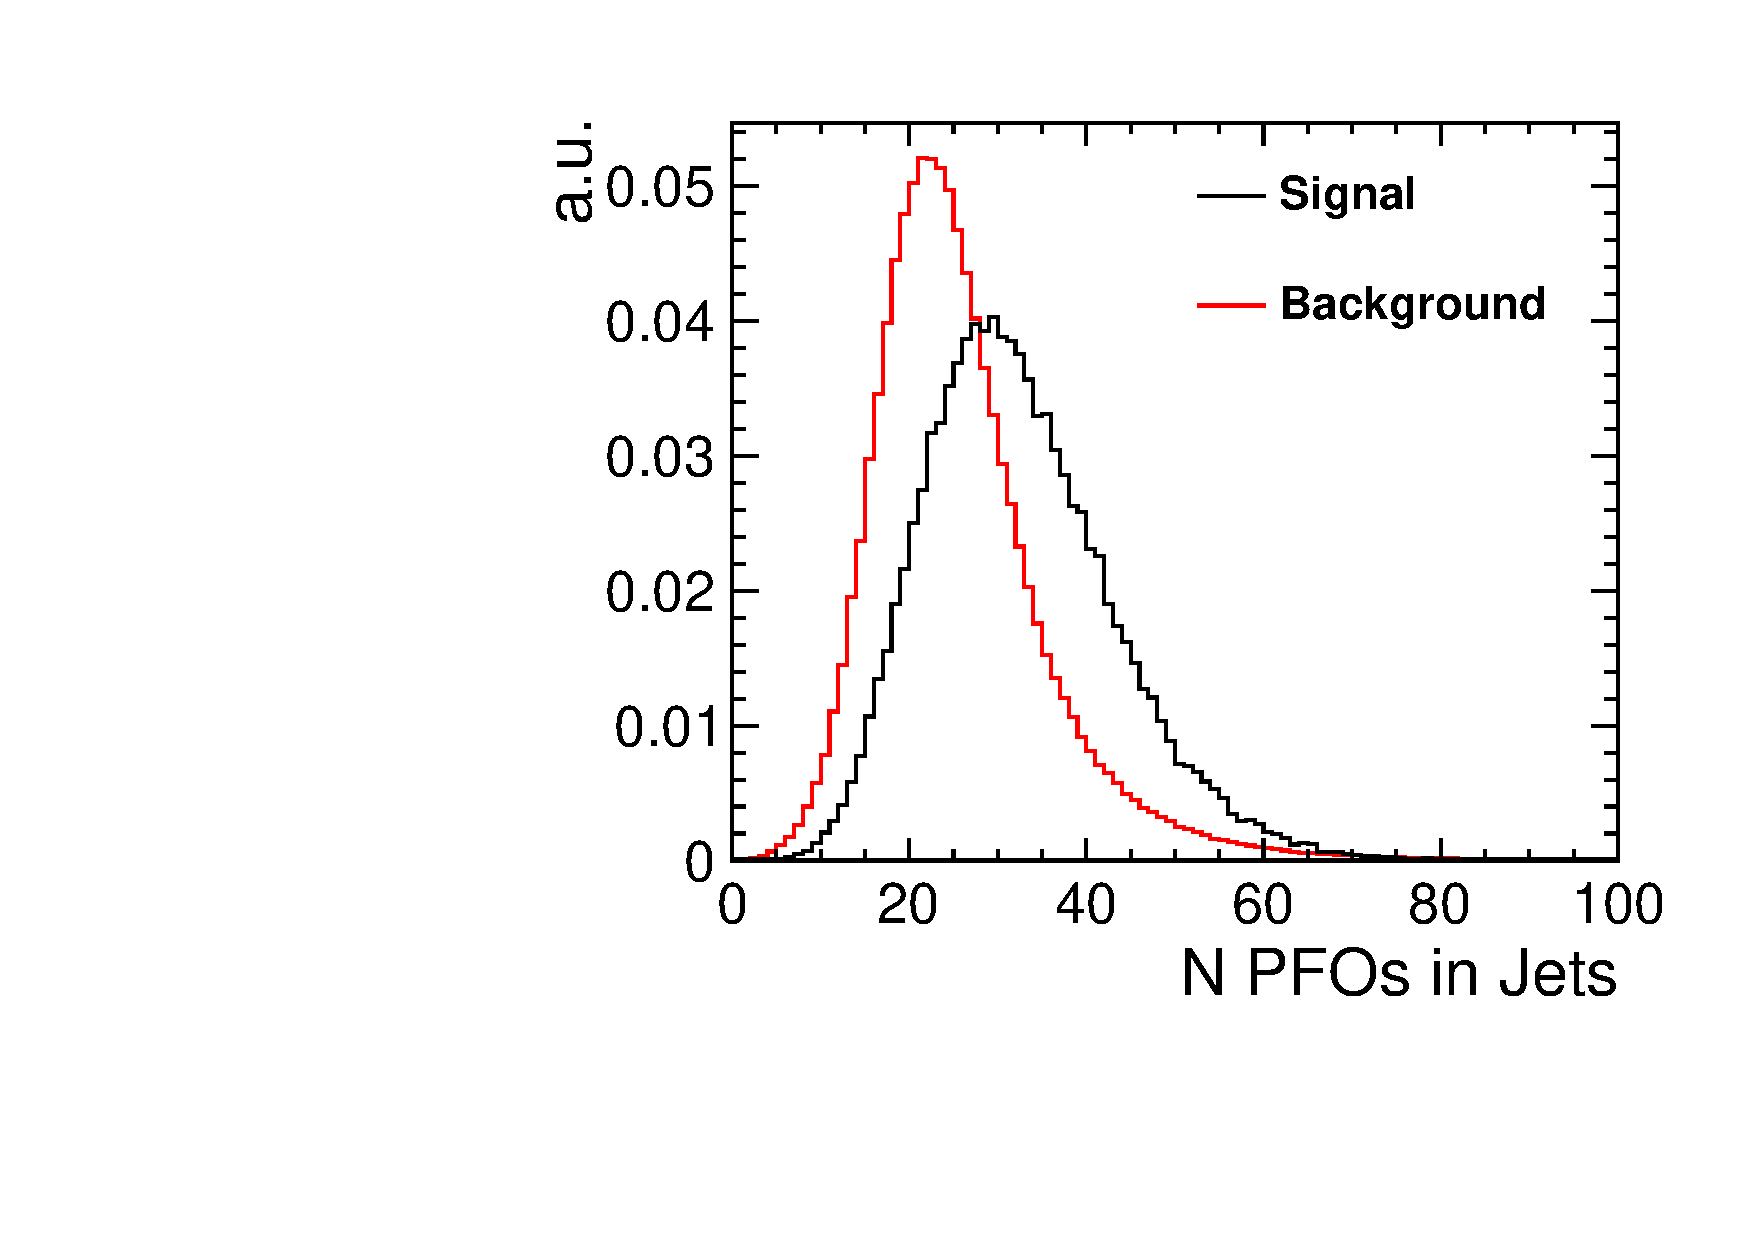
\includegraphics[width=0.75\linewidth]{Appendix/figures/PFOsInJets} 
    \caption{nPFOs assigned to jets} 
    \vspace{4ex}
  \end{subfigure} 
  \begin{subfigure}[]{0.5\linewidth}
    \centering
    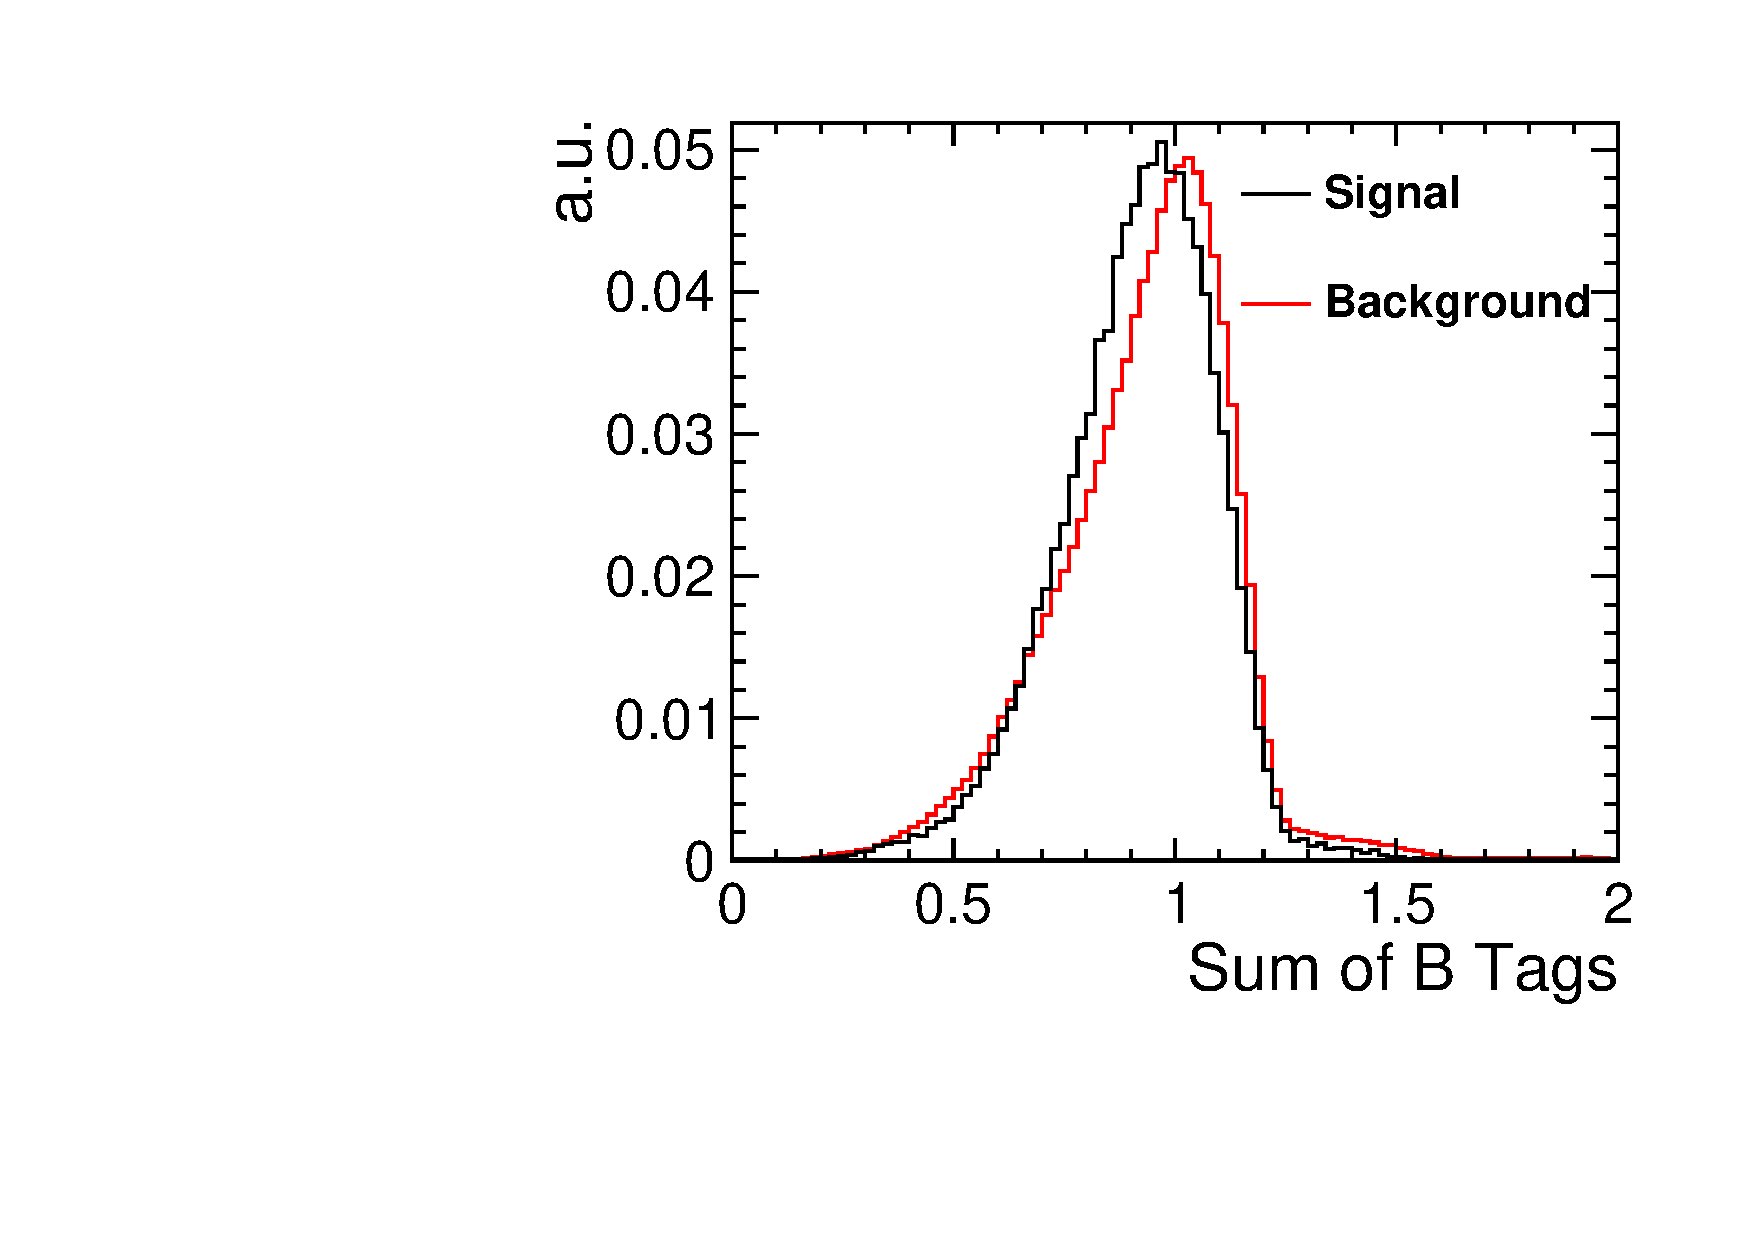
\includegraphics[width=0.75\linewidth]{Appendix/figures/SumBTags} 
    \caption{Sum of two highest b-tags} 
     \vspace{4ex}
 \end{subfigure}%%
  \begin{subfigure}[]{0.5\linewidth}
    \centering
    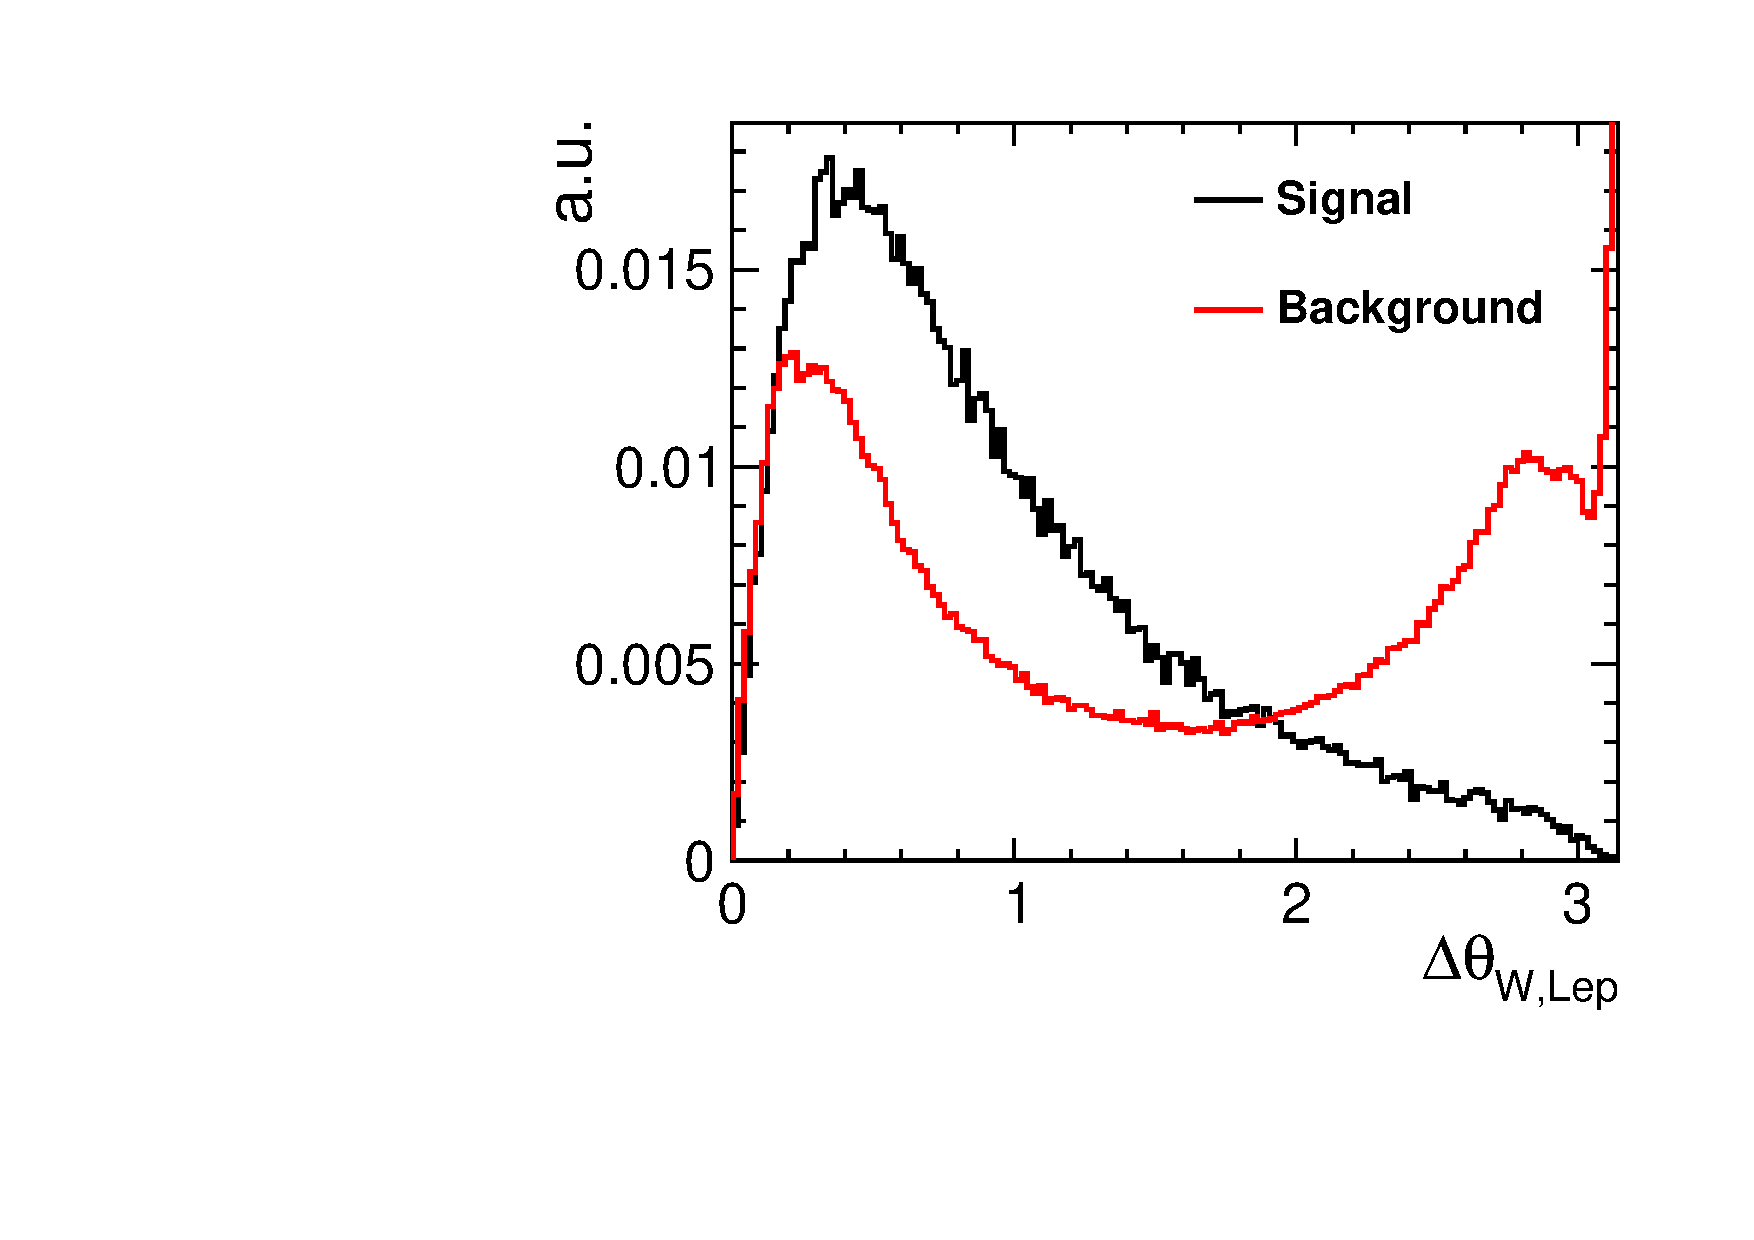
\includegraphics[width=0.75\linewidth]{Appendix/figures/WqqLepAngSep} 
    \caption{Angular Separation of the W and lepton} 
    \vspace{4ex}
  \end{subfigure}
  \begin{subfigure}[]{0.5\linewidth}
    \centering
    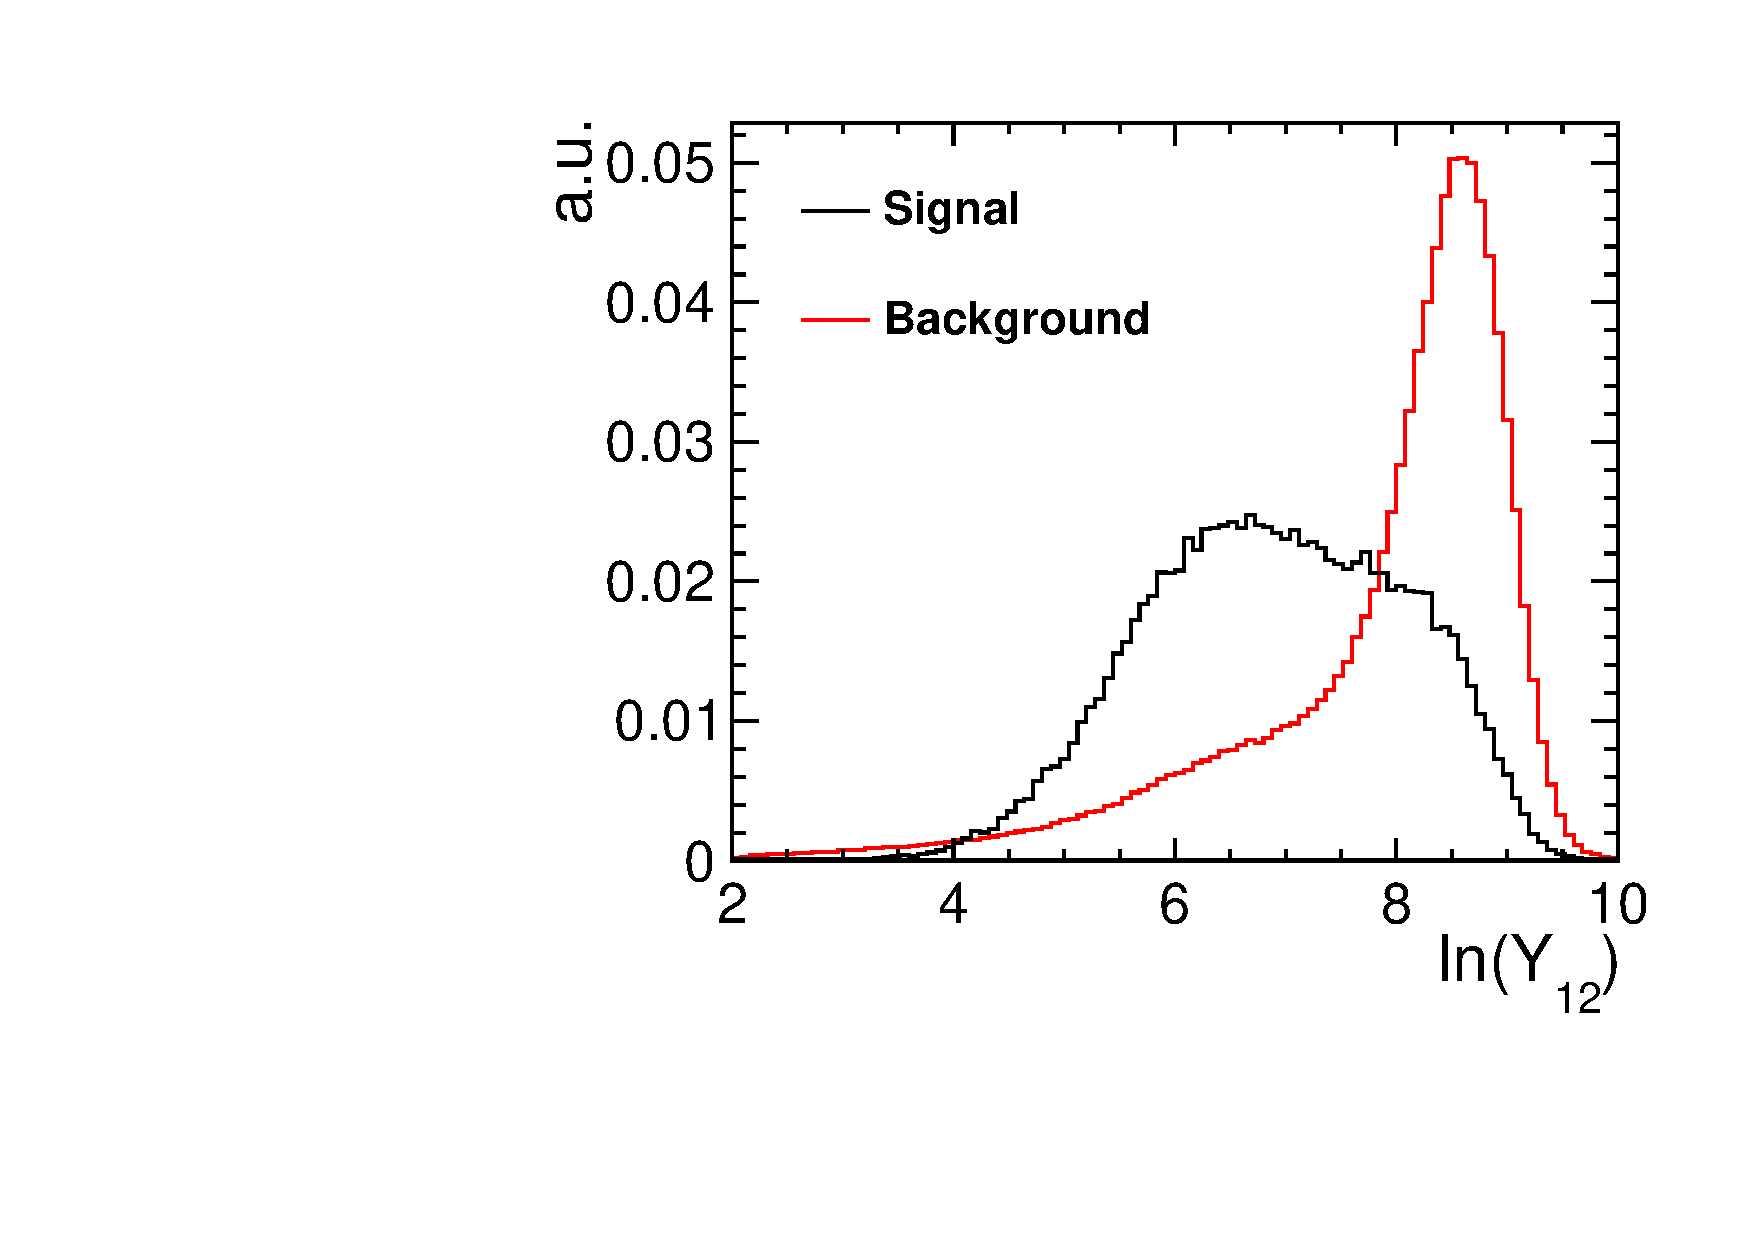
\includegraphics[width=0.75\linewidth]{Appendix/figures/Y12} 
    \caption{Jet Resolution Parameter Y$_{12}$} 
    \vspace{4ex}
  \end{subfigure}%%
\end{figure}


%%%%%%%%%% Appendix %%%%%%%%%%

\end{document} 
